\chapter{Results}
\label{chap:results}

\section{Analytical scope}
\label{sec:results-data-preparation}

The corpus comprises \CoreInteractions{} interactions, \CoreFeedingEvents{} feeding events and \CoreMonitoredRuns{} monitored runs, one per deployment day.

RQ1 to RQ3 report the two phases side by side, so that each effect can be checked with and without assigned roles (Section~\ref{subsec:study-design-deployment}). The phases were not equally long (Table~\ref{tab:phase-corpus}): \CorePOneRecordedHours{} recorded hours against \CorePTwoRecordedHours{}, so Phase~1 contributed more interactions, feeding events, depletion entries and affinity updates, while target-selection logging was almost balanced. Every result is therefore given as a rate on its own denominator, so that unequal exposure between the phases is not mistaken for a difference in effect.

\begin{table}[htbp]
    \centering
    \small
    \caption[Recorded evidence by experimental phase.]{Recorded evidence by experimental phase. A candidate's selection row is logged once the cooldown has passed, and again when its identity, social state or eligibility changes or its score moves by 0.15, but at most once per second. Pings count issued notifications.}
    \label{tab:phase-corpus}
    \begin{tabular}{@{}lrr@{}}
        \toprule
        \textbf{Recorded unit} & \textbf{Phase 1} & \textbf{Phase 2} \\
        \midrule
        Deployment days & \CorePOneDays{} & \CorePTwoDays{} \\
        Recorded hours & \CorePOneRecordedHours{} & \CorePTwoRecordedHours{} \\
        Interactions & \CorePOneInteractions{} & \CorePTwoInteractions{} \\
        Feeding events & \CorePOneFeedingEvents{} & \CorePTwoFeedingEvents{} \\
        Observed depletion entries & \CorePOneDepletionEntries{} & \CorePTwoDepletionEntries{} \\
        Affinity updates & \CorePOneLearningRecords{} & \CorePTwoLearningRecords{} \\
        Target-selection records & \CorePOneSelectionRecords{} & \CorePTwoSelectionRecords{} \\
        Hunger pings / matched messages & \CorePOnePings{}/\CorePOneMessages{} & \CorePTwoPings{}/\CorePTwoMessages{} \\
        \bottomrule
    \end{tabular}
\end{table}

Questionnaire results describe the twelve respondents as a group and are never related statistically to individual feeding or affinity histories, because the logs hold \CoreNamedIdentities{} named identities that cannot be matched one to one with the respondents.

\section{Operational performance}
\label{sec:results-operations}

The vision module processed frames containing a face at a median of \CoreOpsVisionHz{}~Hz, about a third of its 20~Hz scheduler target, and every downstream module received face records at that rate. Of \CoreOpsTurns{} embodied conversational turns, \CoreOpsLLMRequests{} requested a language-model reply: \CoreOpsLLMTurns{} were generated. Generated replies reached speech dispatch a median of \CoreOpsLatencyMedian{}~s after the final transcript (interquartile range \CoreOpsLatencyQOne{}--\CoreOpsLatencyQThree{}~s, maximum \CoreOpsLatencyMax{}~s). The remaining \CoreOpsLocalTurns{} turns needed no generated reply, and \CoreOpsNoResponseTurns{} produced none.

\section{RQ1: Homeostatic functions}
\label{subsec:results-rq1}

\subsection{Monitoring and deficit detection}

The controller recorded \CoreRecordedHours{} hours of resource dynamics over \CoreMonitoredRuns{} runs. Of the \CoreResourceSamples{} recorded samples, \CorePassiveSamples{} were passive updates separated by a median of \CorePassiveGapMedian{}~s; the largest gap, \CorePassiveGapMax{}~s, spans a same-day restart. Monitoring therefore ran whether or not anyone was interacting with the robot.

For all \CoreInteractions{} interactions, the hunger state logged at onset matched the numerical level under the programmed boundaries of 60 points (Full--Hungry) and 25 points (Hungry--Starving). Over passive updates that did not hit the 0 or 100 bound, the observed drain was \CoreObservedDrain{} points per hour against the programmed \CoreNominalDrain{}. The regulator thus tracked the resource as specified and passed the correct hunger state to the executive controller.

\subsection{From deficit to action}

The remote channel shows the gating first. Each of the \CoreTelegramPings{} hunger pings was triggered either by entry into Hungry or by a proactive request issued while Starving, and none came from Full, as the controller is programmed to do. This verifies the gating and says nothing about the response. Whether anyone answered is a question for RQ2.

Face to face, the deficit changed how far interactions progressed. The interaction reached the Engaged state, the controller's completion state, in \CoreFullReachedSSFour{}/\CoreFullInteractions{} Full interactions (\CoreFullSSFourPercent{}\%) and \CoreHungryReachedSSFour{}/\CoreHungryInteractions{} Hungry interactions (\CoreHungrySSFourPercent{}\%), but only \CoreStarvingReachedSSFour{}/\CoreStarvingInteractions{} Starving interactions (\CoreStarvingSSFourPercent{}\%). Full and Hungry barely differed; completion collapsed only below the Starving threshold. That is the pattern expected if the controller reserves its strongest redirection, a feeding request that takes precedence over conversation, for critical deficit. By design, a Starving interaction reaches Engaged only if feeding restores Full and a conversational turn then follows (Algorithm~\ref{alg:executive-control}). The logs do not show at which step the other Starving interactions ended.

\paragraph{Answer to RQ1.} Monitoring ran continuously, deficit detection matched the programmed thresholds in every interaction, and the drive-gated policy (Equation~\ref{eq:executive-policy}) turned deficit into action, both remotely and face to face. Within this deployment, RQ1 is supported on all four functions it names.

\section[RQ2: Recovery-oriented engagement and replenishment]{RQ2: Recovery-oriented engagement\\and replenishment}
\label{subsec:results-rq2}

\subsection{Feeding in response to deficit}

Feeding was uncommon when interactions began in Full and more frequent under deficit (Figure~\ref{fig:results-feeding-observed}). Combining Hungry and Starving, \CoreDeficitFed{}/\CoreDeficitInteractions{} interactions received at least one meal, compared with \CoreFullFed{}/\CoreFullInteractions{} Full interactions. The absolute difference of \CoreFeedingDifference{} percentage points remained positive when any single run or named person was omitted, with leave-one-out differences ranging from \CoreInfluenceLow{} to \CoreInfluenceHigh{} percentage points. These data show a within-deployment association between deficit and feeding.

In Phase~1, \CorePOneDeficitFed{}/\CorePOneDeficitInteractions{} deficit interactions received a meal (\CorePOneDeficitFeedingPercent{}\%), compared with \CorePOneFullFed{}/\CorePOneFullInteractions{} Full interactions (\CorePOneFullFeedingPercent{}\%), a \CorePOneFeedingDifference{} percentage-point difference. In Phase~2, the corresponding rates were \CorePTwoDeficitFed{}/\CorePTwoDeficitInteractions{} (\CorePTwoDeficitFeedingPercent{}\%) and \CorePTwoFullFed{}/\CorePTwoFullInteractions{} (\CorePTwoFullFeedingPercent{}\%), a difference of \CorePTwoFeedingDifference{} percentage points. The Phase~2 Starving proportion rests on only \CorePTwoStarvingInteractions{} interactions, which is why its interval in Figure~\ref{fig:results-feeding-observed} is so wide.

\begin{figure}[htbp]
    \centering
    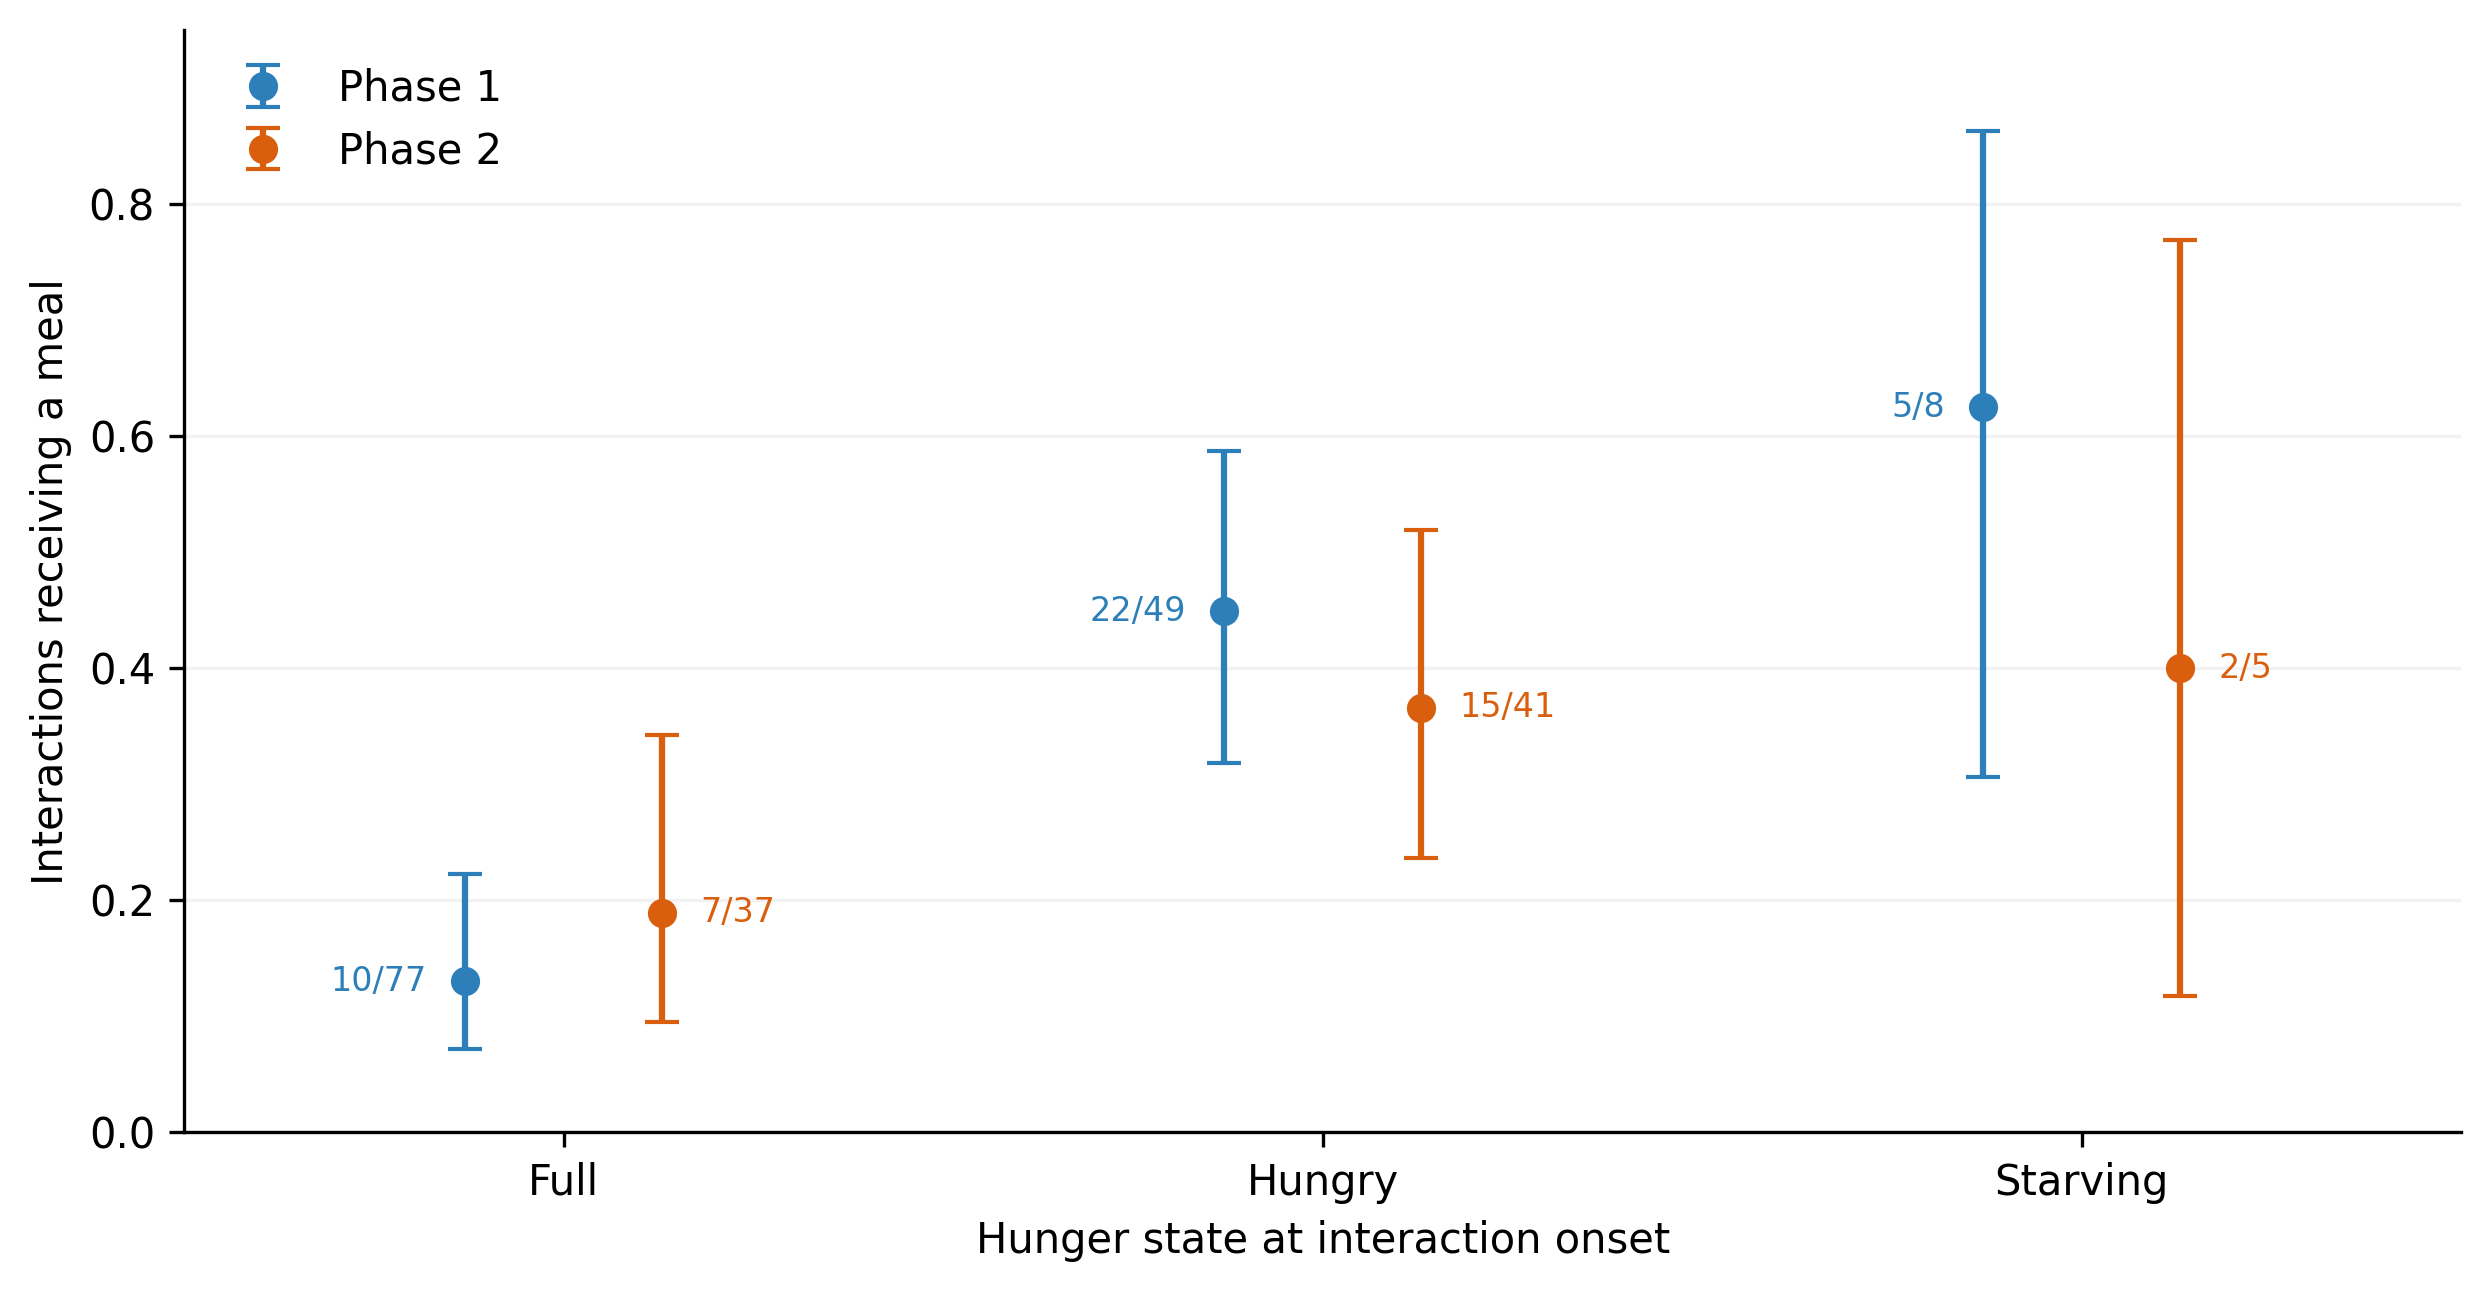
\includegraphics[width=0.86\textwidth,height=0.4\textheight,keepaspectratio]{Results/Figures/feeding-phase-model.png}
    \caption[Observed feeding by hunger state and phase.]{Share of interactions that received at least one meal, by the hunger state in which the interaction began. Points are raw proportions, labels give the exact counts, and bars are 95\% Wilson intervals.}
    \label{fig:results-feeding-observed}
\end{figure}

Raw proportions treat every interaction as independent, yet the same people recur, and a person who feeds readily and happened to attend on a hungry day would inflate the contrast. The mixed-effects logistic model of Equation~\ref{eq:feeding-glmm} (Section~\ref{subsec:statistical-framework}) corrects for this with random intercepts for person and run. It retains \CoreModelN{} interactions from the \CoreModelIdentities{} enrolled participants across \CoreModelRuns{} runs, after the exclusions listed in Section~\ref{subsec:statistical-framework}.

Figure~\ref{fig:results-feeding-model} gives the result. Standardised over the observed people and runs, the probability of a meal rose from \CoreModelPOneFullProbability{}\% in Full to \CoreModelPOneDeficitProbability{}\% in deficit during Phase~1, and from \CoreModelPTwoFullProbability{}\% to \CoreModelPTwoDeficitProbability{}\% during Phase~2. These are differences of \CoreModelPOneRiskDifference{} percentage points (95\% credible interval \CoreModelPOneRiskDifferenceLow{}--\CoreModelPOneRiskDifferenceHigh{}) and \CoreModelPTwoRiskDifference{} points (\CoreModelPTwoRiskDifferenceLow{}--\CoreModelPTwoRiskDifferenceHigh{}). On the odds scale, deficit multiplied the odds of feeding by \CoreModelPOneOR{} in Phase~1 (\CoreModelPOneORLow{}--\CoreModelPOneORHigh{}) and by \CoreModelPTwoOR{} in Phase~2 (\CoreModelPTwoORLow{}--\CoreModelPTwoORHigh{}). Both intervals lie above 1, so the deficit association held after the roles were removed. Its size may have shrunk. Dividing the Phase~2 odds ratio by the Phase~1 odds ratio gives \CoreModelPhaseORRatio{}, but the interval (\CoreModelPhaseORRatioLow{}--\CoreModelPhaseORRatioHigh{}) spans 1, so the data neither show a change between phases nor rule one out.

\begin{figure}[htbp]
    \centering
    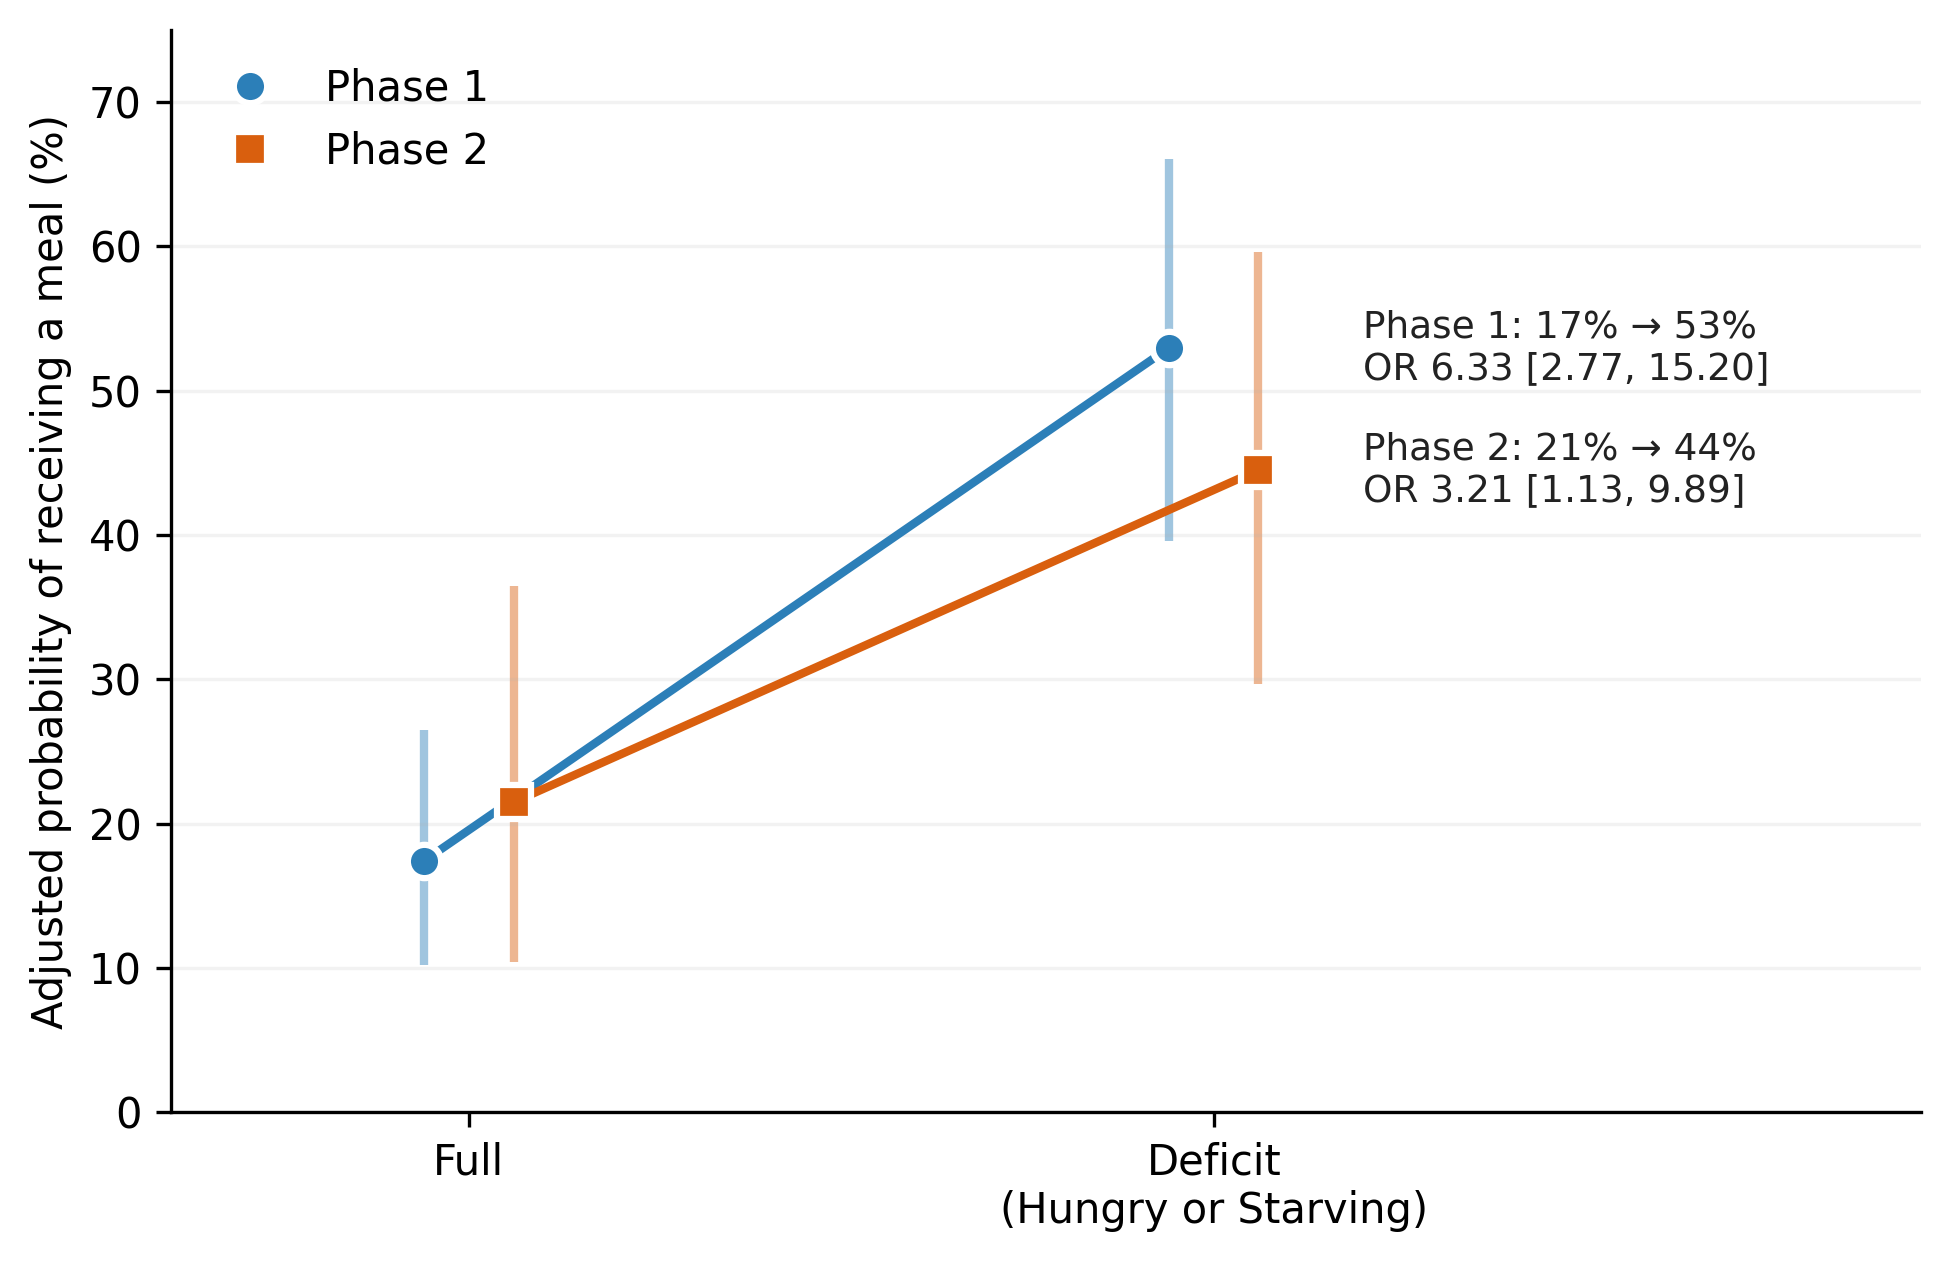
\includegraphics[width=0.7\textwidth,height=0.4\textheight,keepaspectratio]{Results/Figures/feeding-model.png}
    \caption[Mixed-effects model of feeding.]{Probability that an interaction received a meal, as estimated by the mixed-effects logistic model of Equation~\ref{eq:feeding-glmm} after accounting for repeated people and runs. Deficit pools Hungry and Starving. Each line is one phase, and its slope is the deficit effect; bars are 95\% credible intervals, and the labels give the two probabilities and the deficit odds ratio (OR) with its interval. Appendix~\ref{app:feeding-model} plots every fitted term.}
    \label{fig:results-feeding-model}
\end{figure}

Figure~\ref{fig:results-feeding-model} shows two rising lines, with the Phase~1 line steeper. The probability of a meal in a full robot is similar in both phases, so the phases differ in how far deficit lifts feeding, not in how often a satisfied robot is fed. In Phase~1 the intervals for Full and deficit do not overlap. In Phase~2 they touch at their edges, since that phase has fewer interactions. The contrast itself still excludes zero (\CoreModelPTwoRiskDifferenceLow{}--\CoreModelPTwoRiskDifferenceHigh{} points), because it is computed draw by draw from the same posterior, so the uncertainty the two probabilities share cancels out.

The random-intercept standard deviations were \CoreModelIdentitySD{} on the log-odds scale for identity (95\% credible interval \CoreModelIdentitySDLow{}--\CoreModelIdentitySDHigh{}) and \CoreModelRunSD{} for run (\CoreModelRunSDLow{}--\CoreModelRunSDHigh{}). People differed more than days did, and the run interval reaches almost to zero; both intervals are broad. Figure~\ref{fig:results-feeding-glmm} in Appendix~\ref{app:feeding-model} shows where that spread comes from. Most identity intercepts straddle zero. One person (P06) feeds more than average, with an interval that just clears zero, and the lowest intercepts (P03 and P11) lean the other way without clearly leaving it. People with only two to four interactions are pulled toward zero (partial pooling). The run intercepts all sit close to zero, so no single deployment day drives the deficit association. With \CoreModelIdentities{} participants and \CoreModelRuns{} runs these spreads are imprecise and are not meant to rank people.

Sampling produced no divergent transitions, all $\hat R$ values were at most \CoreModelMaxRhat{}, and the minimum bulk effective sample size was \CoreModelMinESS{}. The posterior predictive 95\% interval of \CoreModelPPFeedingLow{}--\CoreModelPPFeedingHigh{} feeding interactions contained the \CoreModelObservedFeeding{} observed among the retained records.

\subsection{Meal choice under deficit}

Meals grew larger as the deficit deepened, which is the direction regulation requires (Table~\ref{tab:meal-choice}). At the moment of feeding, \CoreStarvingLargeMeals{} of \CoreStarvingMeals{} Starving meals were large and none was small. Hungry meals were more mixed, and half of the \CoreFullMeals{} meals delivered while Full were small.

The \CoreFeedingEvents{} meals supplied \CoreNominalMealPoints{} nominal points but increased the recorded resource by \CoreAcceptedMealPoints{} points because replenishment was clipped at 100. Of the \CoreClippedPoints{} clipped points, \CoreClippedPointsFull{} came from meals given while Full. Meals given under deficit lost only the remaining few points to the cap, so they restored the resource almost point for point.

\begin{table}[htbp]
    \centering
    \small
    \caption{Nominal meal choice by hunger state immediately before the feeding event.}
    \label{tab:meal-choice}
    \begin{tabular}{@{}lrrr@{}}
        \toprule
        \textbf{State} & \textbf{Small (10)} & \textbf{Medium (25)} & \textbf{Large (45)} \\
        \midrule
        Full     & \CoreFullSmallMeals     & \CoreFullMediumMeals     & \CoreFullLargeMeals \\
        Hungry   & \CoreHungrySmallMeals   & \CoreHungryMediumMeals   & \CoreHungryLargeMeals \\
        Starving & \CoreStarvingSmallMeals & \CoreStarvingMediumMeals & \CoreStarvingLargeMeals \\
        \bottomrule
    \end{tabular}
\end{table}

\subsection{Starving episodes and observed occupancy}

The logged levels show \CoreDepletionEpisodes{} entries into Starving: \CoreInteractionCostEpisodes{} followed interaction cost and \CorePassiveDrainEpisodes{} followed passive drain. Phase~1 contained \CorePOneDepletionEntries{} entries and Phase~2 \CorePTwoDepletionEntries{}, and every one of them later reached Full through feeding. This endpoint counts episodes, not interactions: \CoreStarvingOnsetUnfed{} of the \CoreStarvingInteractions{} individual interactions that began in Starving received no meal.

Recovery time varied by almost three orders of magnitude (Figure~\ref{fig:results-recovery-episodes}). Across the \CoreDepletionEpisodes{} depletion entries, the median time from crossing into Starving to reaching Full was \CoreRecoveryMedianSeconds{}~s, with a range of \CoreRecoveryMinimumSeconds{}--\CoreRecoveryMaximumSeconds{}~s. Entries caused by interaction cost recovered quickly: the Phase~1 median was \CorePOneInteractionCostMedian{}~s across \CorePOneInteractionCostEpisodes{} episodes, and the Phase~2 median was \CorePTwoInteractionCostMedian{}~s across \CorePTwoInteractionCostEpisodes{} episodes. The two passive-drain episodes lasted \CorePassiveDrainShorter{} and \CorePassiveDrainLonger{}~s.

\begin{figure}[htbp]
    \centering
    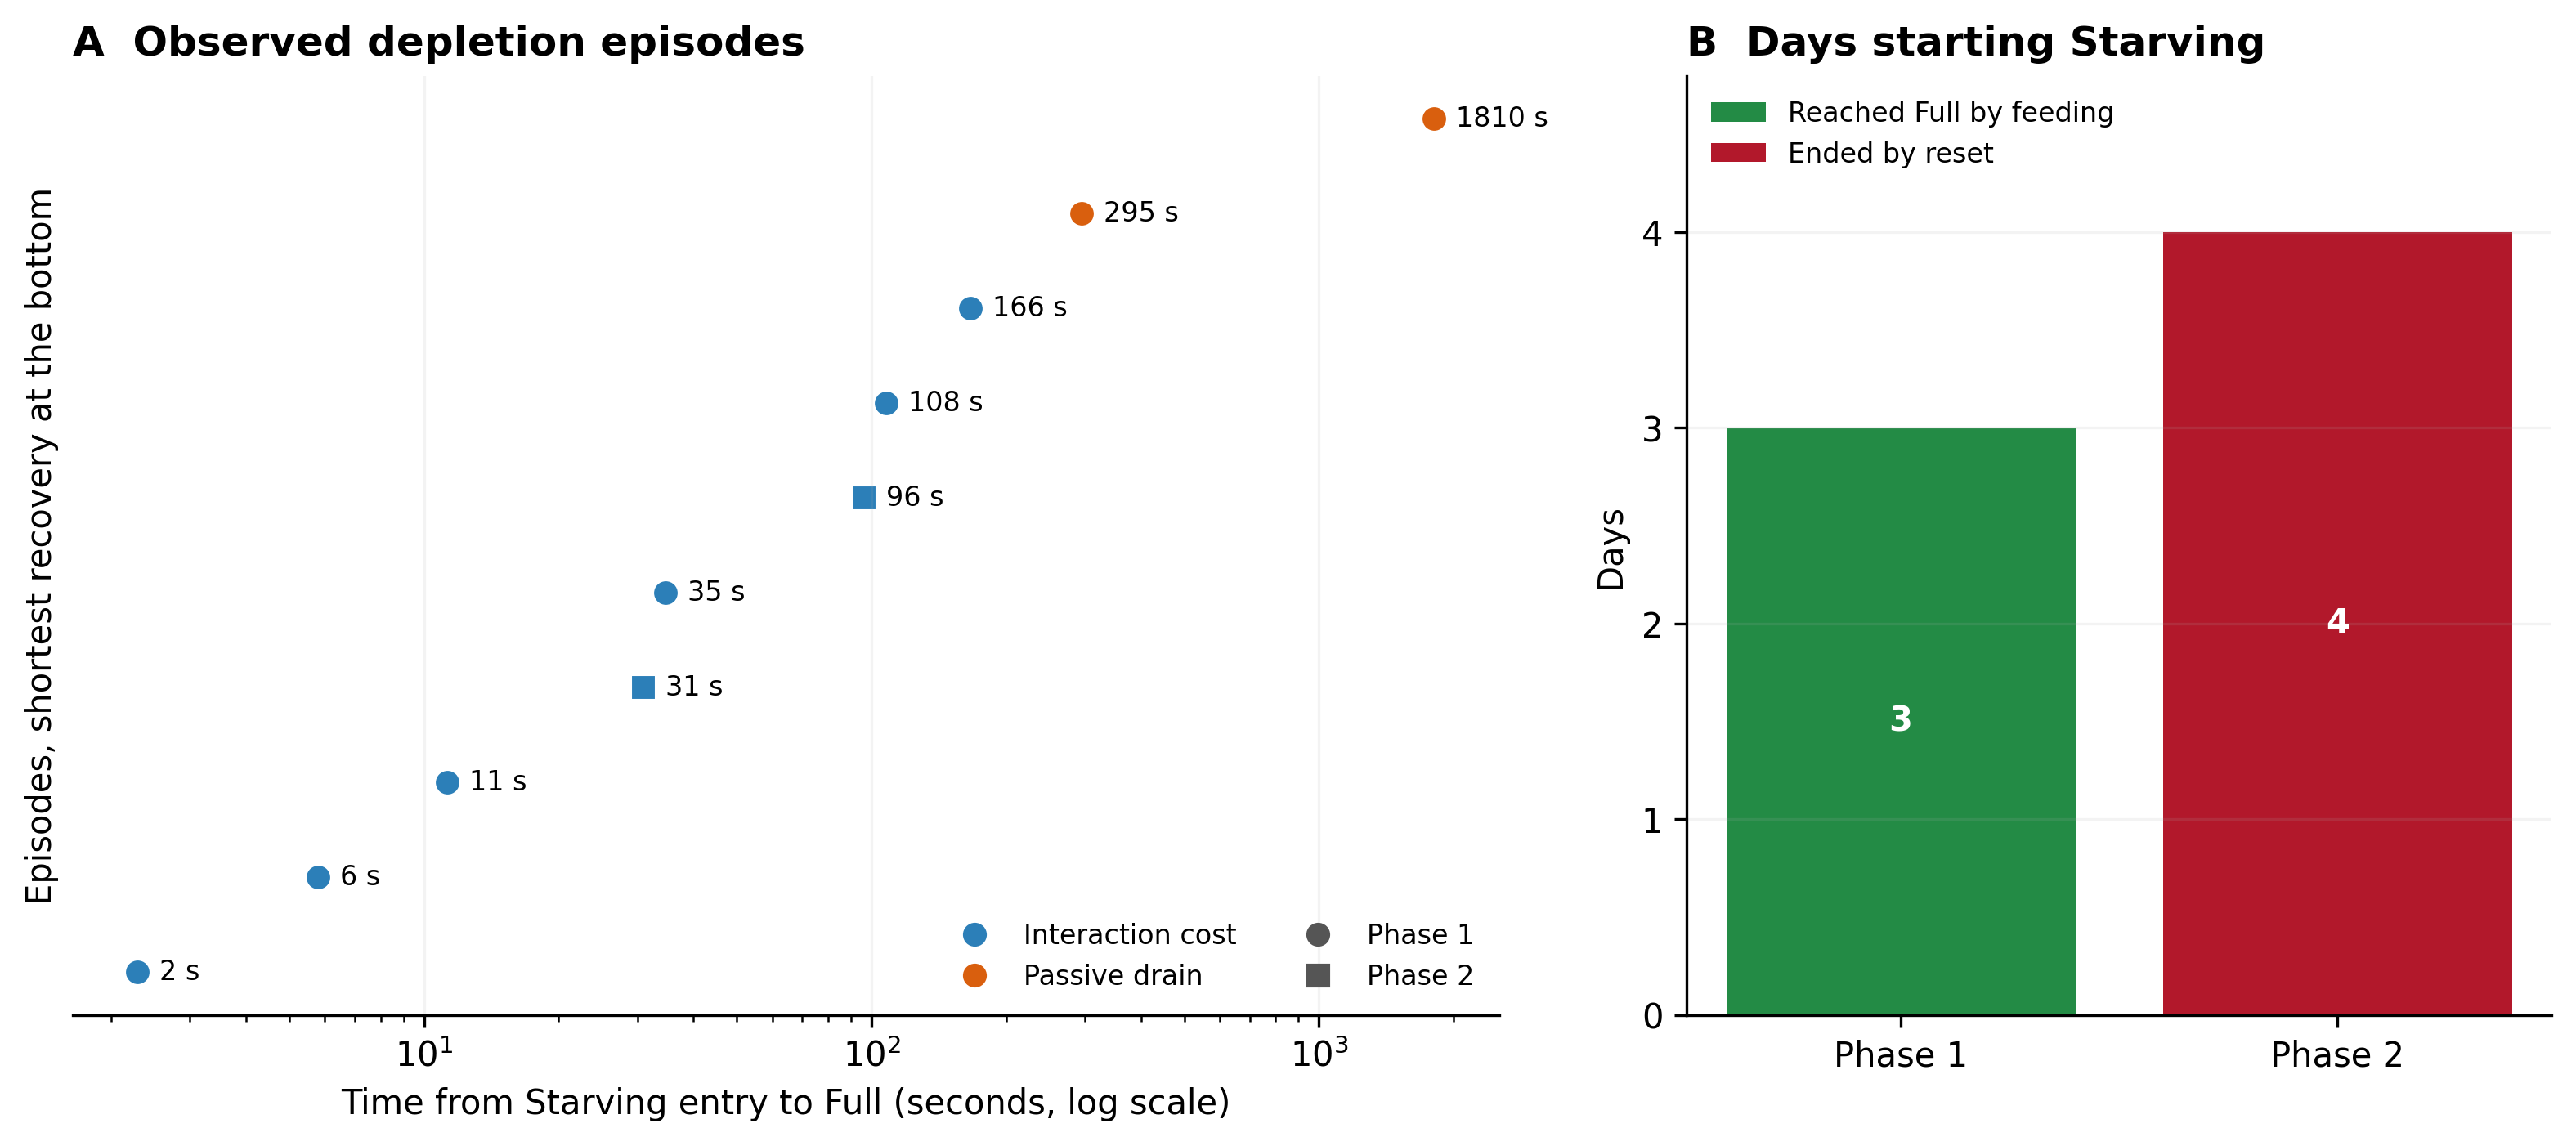
\includegraphics[width=0.95\textwidth,height=0.48\textheight,keepaspectratio]{Results/Figures/recovery-episodes.png}
    \caption[Recovery of observed Starving episodes and of days starting Starving.]{How long the robot stayed in critical deficit before feeding restored Full, the replenishment evidence for RQ2. Panel A plots time to Full for each of the \CoreDepletionEpisodes{} observed entries into Starving, coloured by what caused the entry, with marker shape giving the phase. Its logarithmic axis keeps recoveries of seconds and of hours on one scale. Panel B treats separately the \CoreStartupSegments{} run-start segments that were already Starving when recording began.}
    \label{fig:results-recovery-episodes}
\end{figure}

A further \CoreStartupSegments{} run-start segments were already Starving when recording began. The \CorePOneStartupSegments{} in Phase~1 reached Full through feeding, whereas all \CorePTwoStartupSegments{} in Phase~2 ended through a mode reset.

Starving occupied \CoreStarvingMinutes{} minutes, \CoreStarvingPercent\% of recorded run time, and \CoreStarvingWithoutInitial\% once the initial Starving portion of run-start segments is excluded. Most of that time came from the two passive-drain episodes, during which nobody was present; they account for \CorePassiveStarvingShare{}\% of it. Figure~\ref{fig:results-drive-timeline} shows this concentration and marks feeding and mode events separately.

\begin{figure}[htbp]
    \centering
    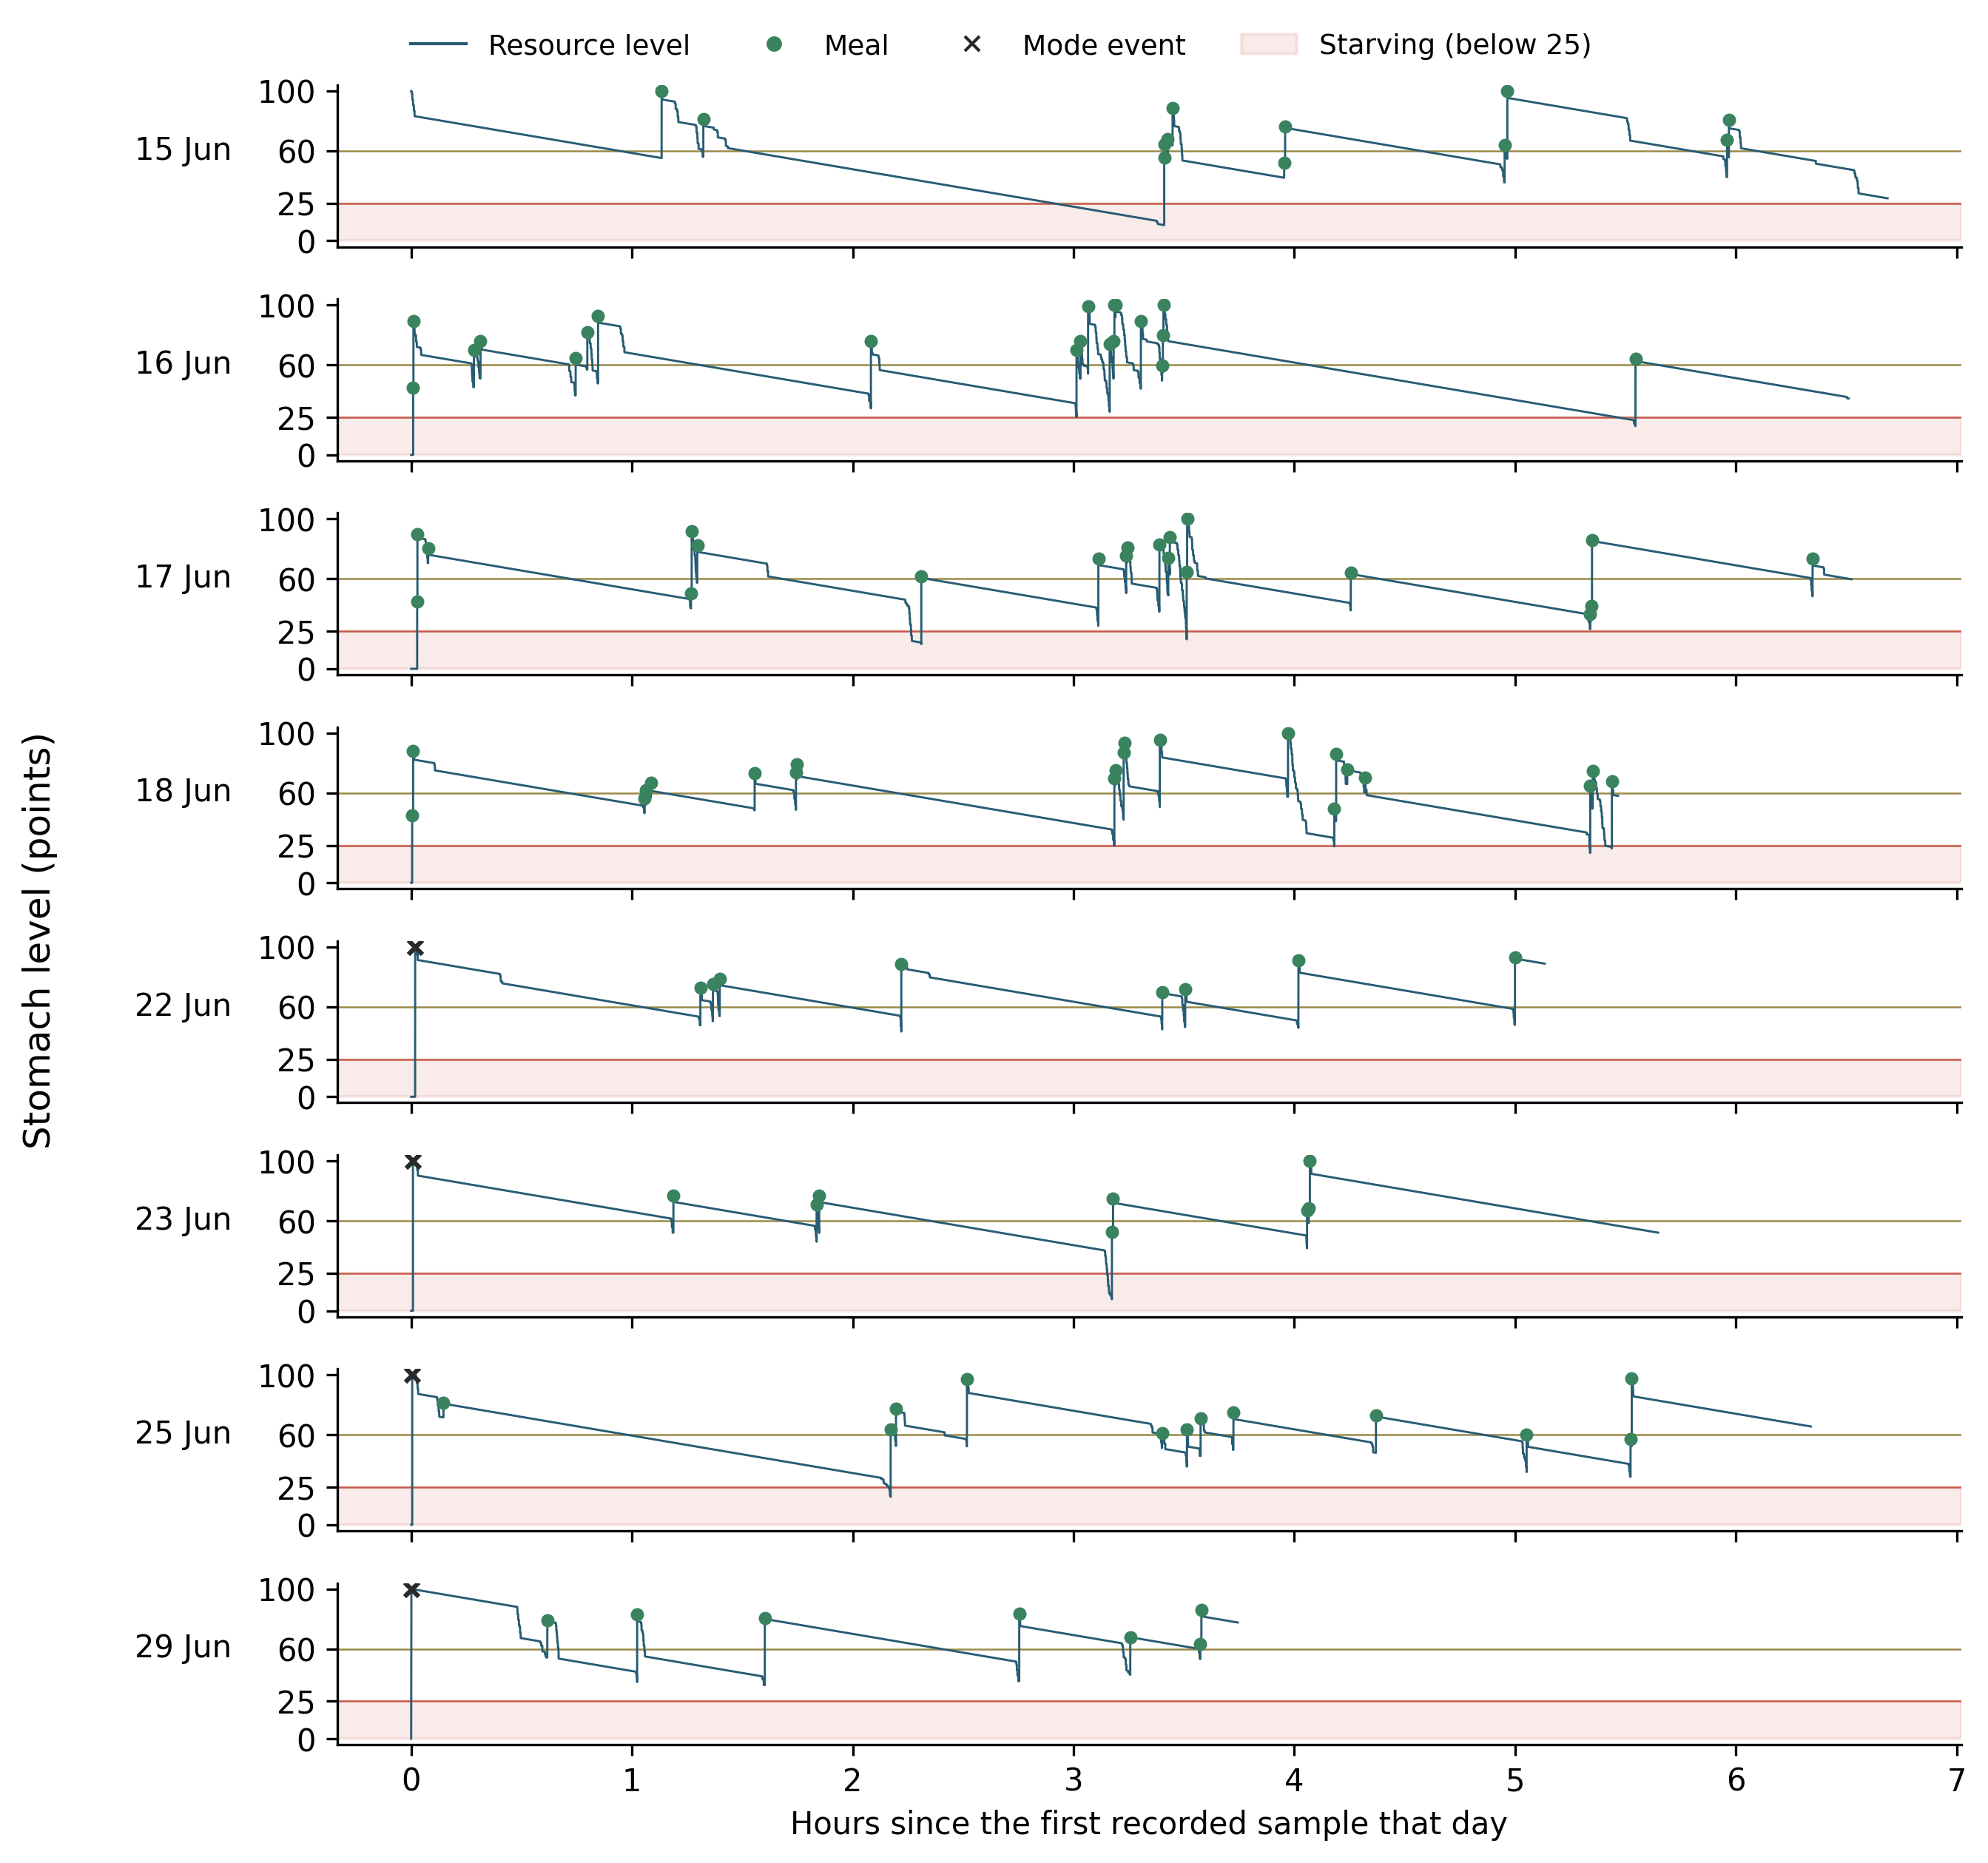
\includegraphics[width=0.84\textwidth,height=0.52\textheight,keepaspectratio]{Results/Figures/drive-timeline.png}
    \caption[Recorded orexigenic-drive dynamics.]{The resource level as logged on each of the eight deployment days, with hours counted from the day's first sample. Passive drain appears as the long downward slopes, action costs as small steps, and meals (green points) as jumps upward. Crosses mark mode events and the shaded band is the Starving region below 25 points.}
    \label{fig:results-drive-timeline}
\end{figure}

\subsection{Remote signalling}

Within 15 minutes of a logged hunger ping, a user message followed in \CoreTelegramMessages{}/\CoreTelegramPings{} cases: \CorePOneMessages{}/\CorePOnePings{} in Phase~1 and \CorePTwoMessages{}/\CorePTwoPings{} in Phase~2. The two phases sent different kinds of notification, because Hungry-entry notices were first sent on 18 June 2026. Phase~1 pings were mostly proactive Starving requests (\CorePOneStarvingProactivePings{}, with \CorePOneStarvingProactiveMessages{} matches) and only \CorePOneHungryEntryPings{} Hungry-entry notices, none of them answered. Phase~2 pings were mostly Hungry-entry notices (\CorePTwoHungryEntryPings{}, with \CorePTwoHungryEntryMessages{} matches) and \CorePTwoStarvingProactivePings{} proactive Starving requests (\CorePTwoStarvingProactiveMessages{} matches). Phase~2's higher reply rate therefore comes with a different mix of notifications, so the two rates do not compare like with like. The \CoreTelegramMessages{} matched messages arrived a median of \CoreTelegramLatencyMedian{}~s after their ping, the fastest after \CoreTelegramLatencyMin{}~s and the slowest after \CoreTelegramLatencyMax{}~s.

\paragraph{Answer to RQ2.} Feeding was associated with deficit in both phases, including after roles were lifted, but recovery was not reliable after every request. Meals grew with the deficit, and every observed depletion entry returned to Full. Yet \CoreStarvingOnsetUnfed{} of the \CoreStarvingInteractions{} Starving-onset interactions went unfed, only \CoreTelegramMessages{} of \CoreTelegramPings{} remote pings drew a reply, and every Phase~2 segment that started Starving ended by a mode reset instead of feeding. The association supports recovery-oriented engagement within this deployment, without establishing a causal effect of hunger expression.

\section{RQ3: Adaptive regulatory memory and its expression}
\label{subsec:results-rq3}

\subsection{Affinity update verification}

Recomputing each of the \CoreLearningRecords{} logged learning records with the affinity rule of Equation~\ref{eq:affinity-update} reproduced its value with no numerical discrepancy and its outcome label in every case. The controller stores affinity under the exact spelling the face recogniser returns, so \CoreSplitPeople{} people were held as several independent entries (for example, two spellings of one given name), whereas the delivered log carries one name per person. I separated the entries by following each update's starting value. This gives \CoreMemoryKeys{} memory keys, each matching a stored key exactly in number of updates and final value. The event table omits the update counter that decides whether a positive update is a person's first, so I checked all \CoreUnobservedCounterUpdates{} positive events against both permitted branches. \CoreFirstUpdateBranches{} of them match only the first-update branch.

Affinity was formed in both phases: \CorePOneLearningRecords{} updates were logged in Phase~1 and \CorePTwoLearningRecords{} in Phase~2. Final stored affinity spanned \CoreFinalAffinityMinimum{} to \CoreFinalAffinityMaximum{} across the \CoreMemoryKeys{} memory keys, with a median of \CoreFinalAffinityMedian{} (Figure~\ref{fig:results-affinity-trajectories}).

\begin{figure}[htbp]
    \centering
    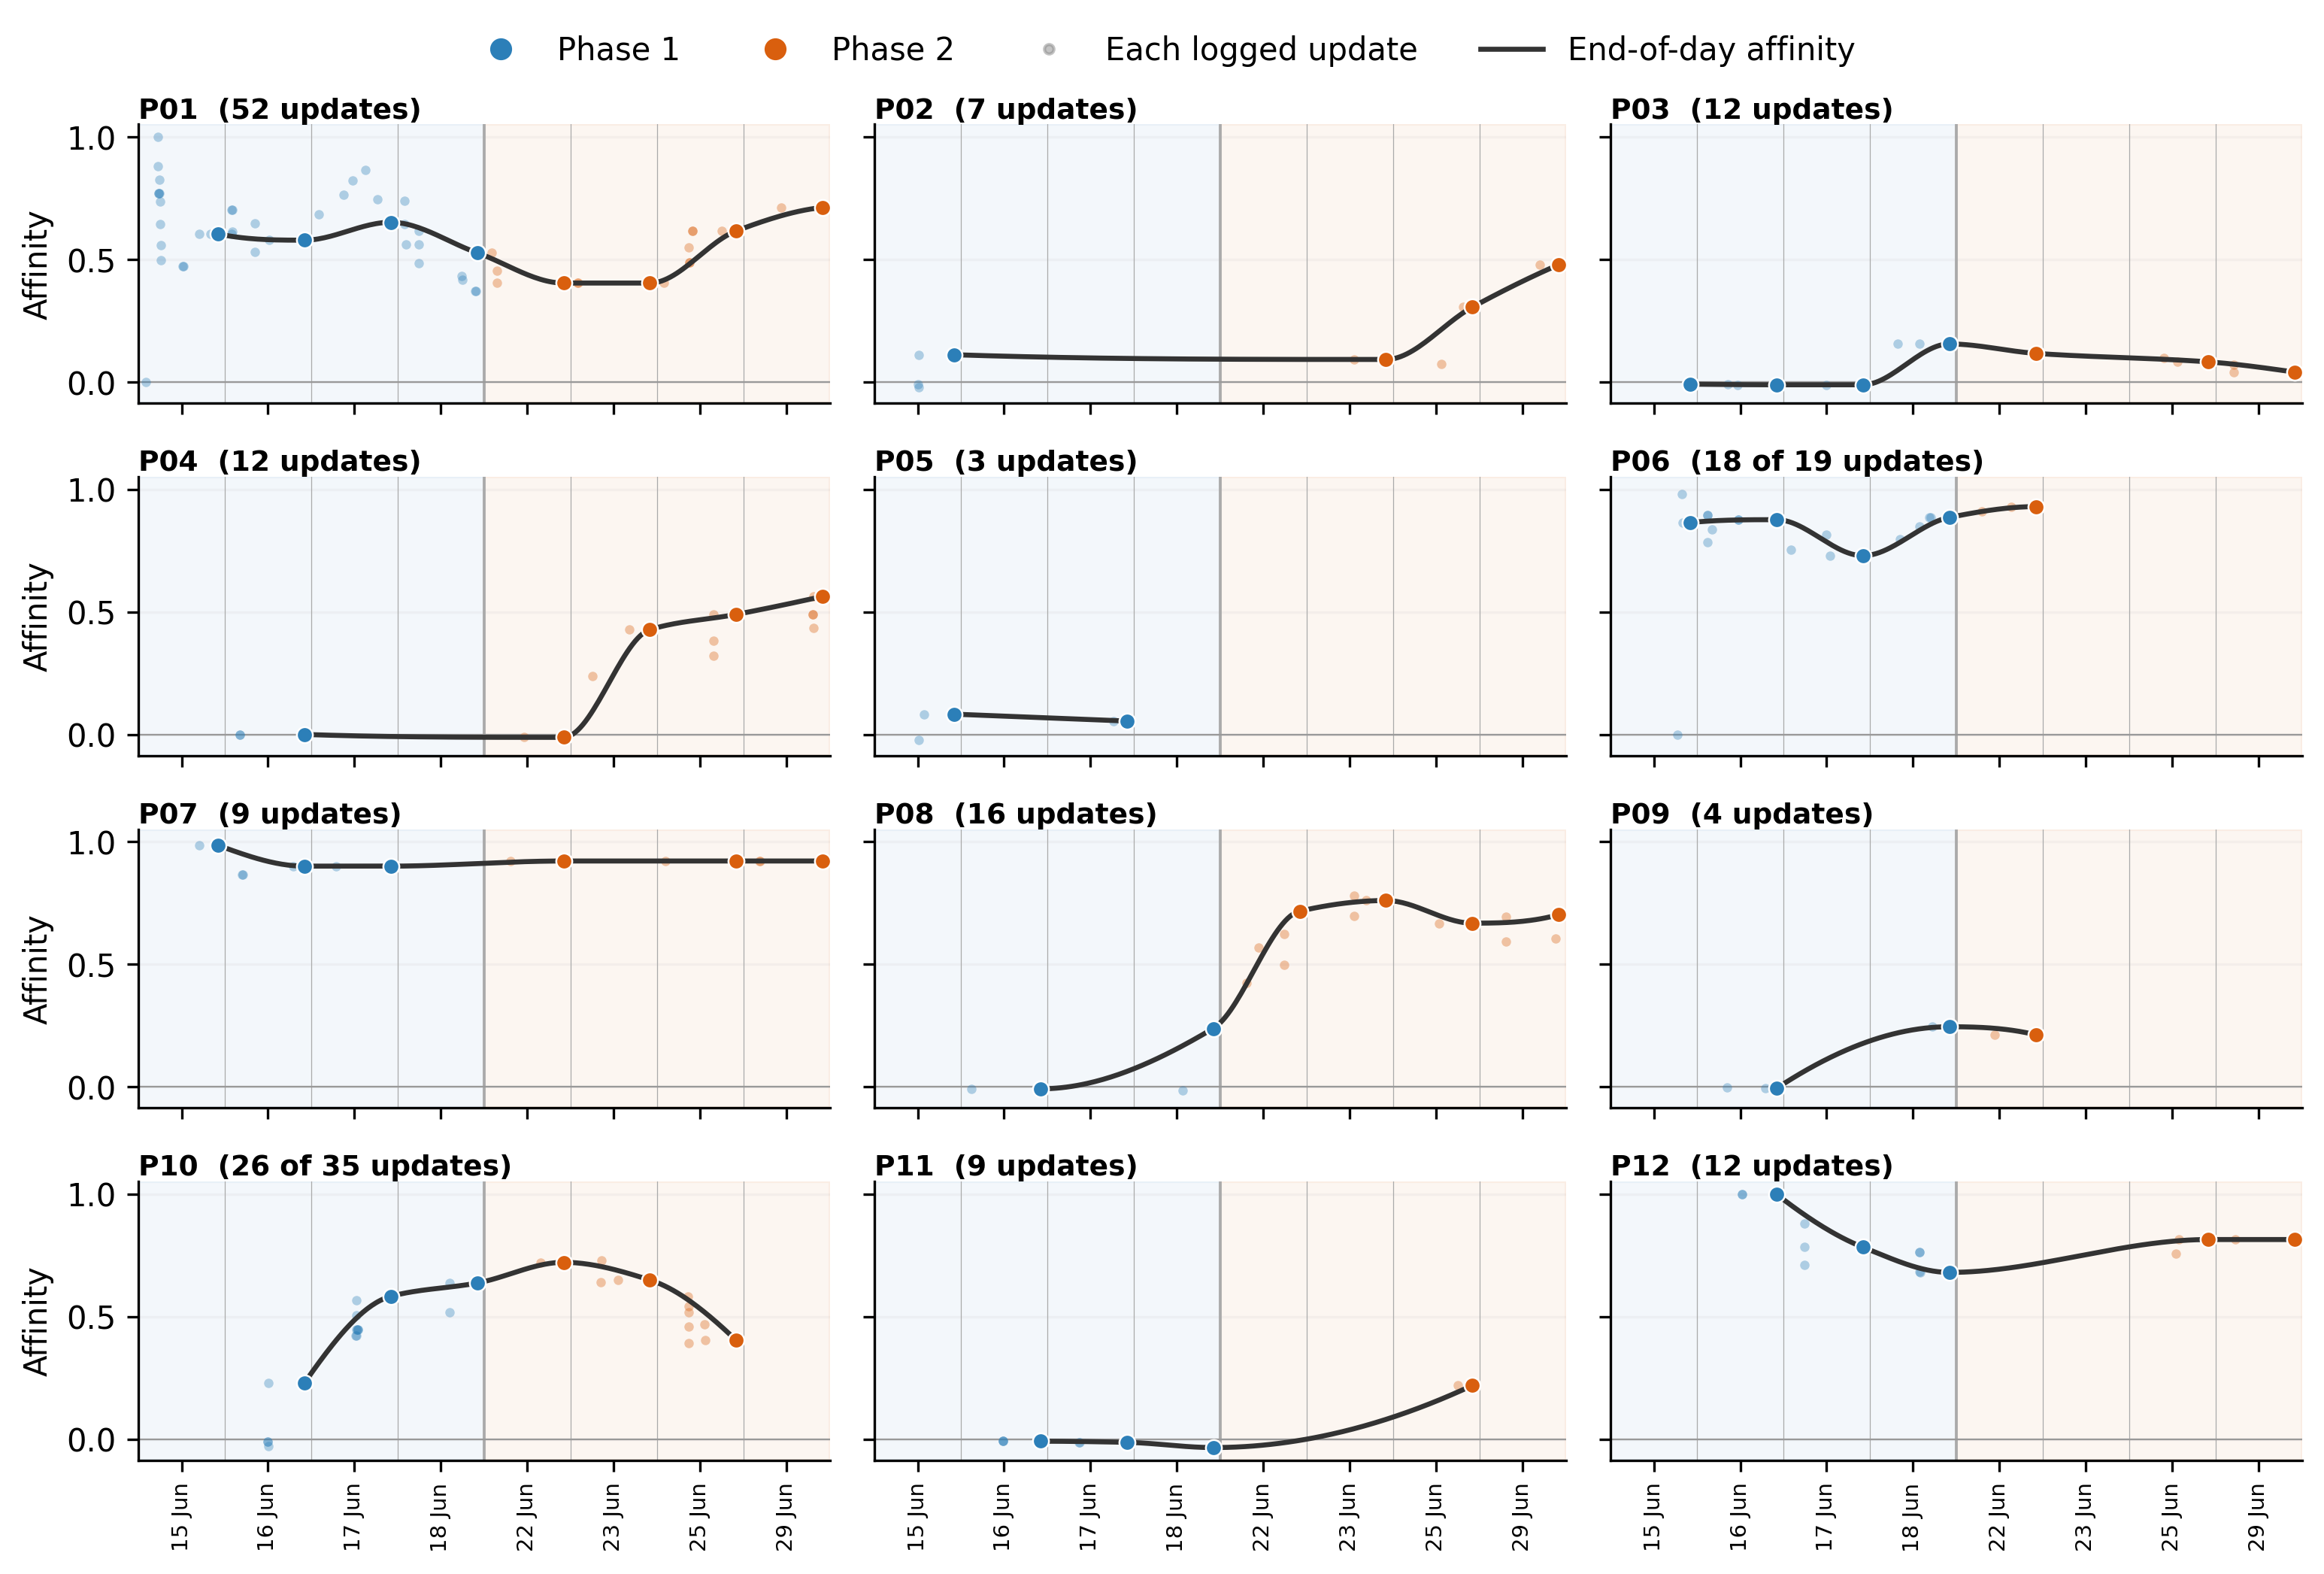
\includegraphics[width=0.92\textwidth,height=0.56\textheight,keepaspectratio]{Results/Figures/affinity-trajectories.png}
    \caption[Logged affinity histories by participant.]{How the robot's learned affinity for each of the \CoreAffinityShownPeople{} enrolled participants moved with the logged updates, the encoding half of RQ3. The \CoreAffinityOmittedPeople{} logged identities outside the roster have \CoreAffinityOmittedUpdates{} updates between them and are not drawn. Faint dots mark every update. A meal lifts affinity and an unrewarded approach lowers it (Equation~\ref{eq:affinity-update}), so single updates zigzag within a day; the line joins the end-of-day value with a smooth monotone curve. For people held under several spellings, the panel shows only the entry with the most updates, and the other entries add \CoreAffinityOtherEntryUpdates{} updates that are not drawn. Each deployment day gets an equal slot, marker colour gives the phase, and the heavier vertical line marks the phase boundary. Positive values lower that person's eligibility threshold, and Figure~\ref{fig:results-affinity-eligibility} shows where this changed a decision.}
    \label{fig:results-affinity-trajectories}
\end{figure}

\subsection{Expression in recorded eligibility decisions}

For each of \CoreSelectionRecords{} named target-selection records, the logged effective threshold equalled
\(
\max(0.50,\theta_s-0.15A_i)
\)
and the eligibility flag agreed with the comparison between IPS and that threshold. Against the neutral-affinity threshold, \CoreEnabledRecords{} records were eligible with their recorded affinity but would have stayed below it; \CoreRestrictedRecords{} record showed the reverse under negative affinity, and every other record received the same decision under both thresholds (Figure~\ref{fig:results-affinity-eligibility}).

Of the records that affinity made eligible, \CorePOneEnabledByAffinity{} fell in Phase~1 and \CorePTwoEnabledByAffinity{} in Phase~2; the single restriction occurred in Phase~1. Affinity therefore kept changing eligibility decisions after the roles were removed. These counts are logged records, not distinct approaches, since one approach opportunity can be logged several times (Table~\ref{tab:phase-corpus}).

\begin{figure}[htbp]
    \centering
    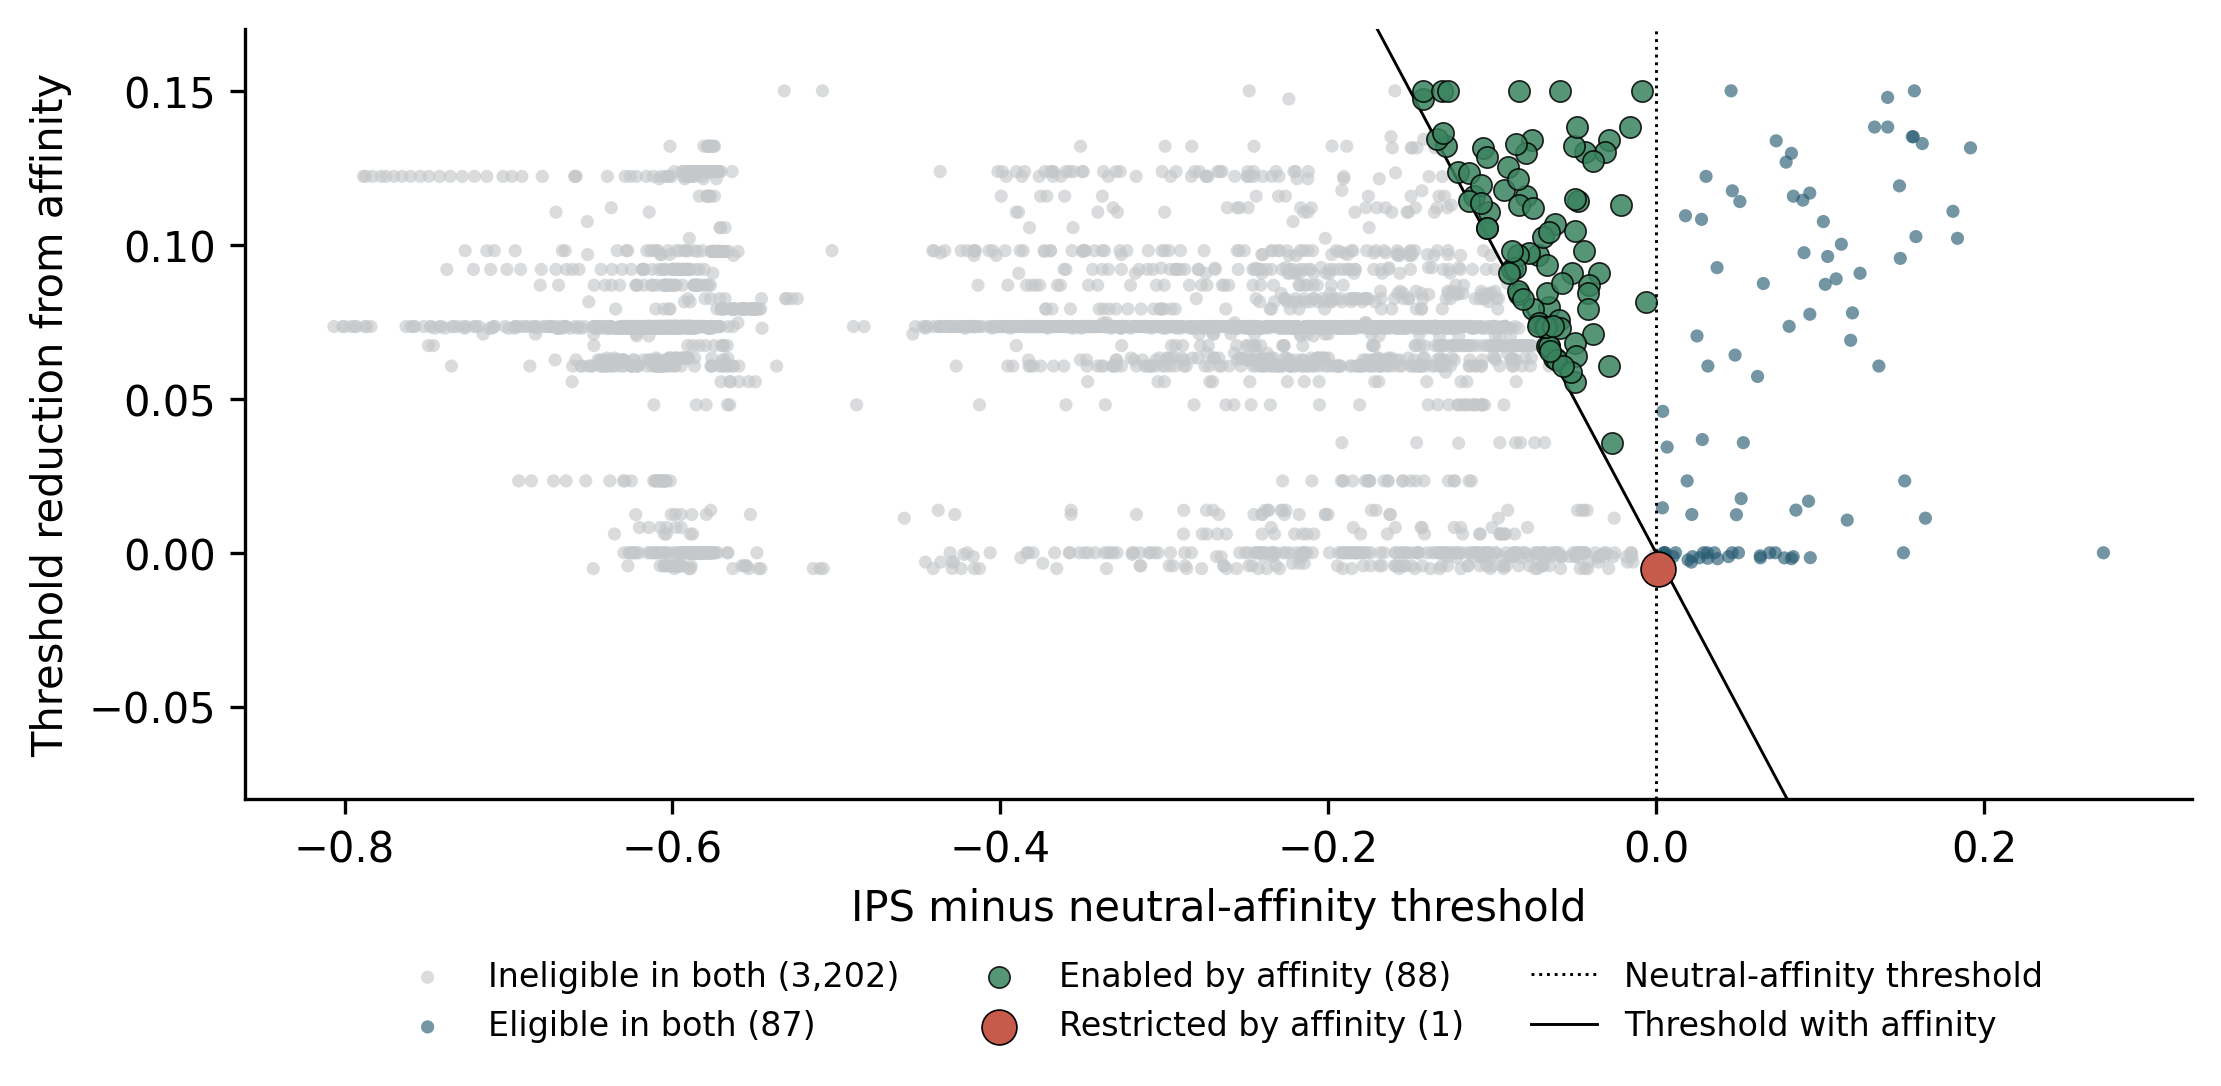
\includegraphics[width=0.86\textwidth,height=0.48\textheight,keepaspectratio]{Results/Figures/affinity-eligibility.png}
    \caption[Affinity and recorded eligibility.]{Where learned affinity decided whether the robot could approach someone, the expression half of RQ3. Each point is one of \CoreSelectionRecords{} named target-selection records. The horizontal axis gives how far its Interaction Priority Score fell above or below the threshold at neutral affinity, and the vertical axis gives how much affinity lowered that threshold. Records right of the diagonal were eligible. The \CoreEnabledRecords{} green records passed only because of affinity, and the single red record was blocked by it. Grey and blue records would have been decided the same way without affinity.}
    \label{fig:results-affinity-eligibility}
\end{figure}

\paragraph{Answer to RQ3.} The adaptive memory stored attributed regulatory outcomes exactly as programmed, and the stored state changed eligibility decisions in both phases. RQ3 is supported for both encoding and expression.

\section{RQ4: Perceived naturalness and social embeddedness}
\label{subsec:results-rq4}

RQ4 rests on the questionnaire of Section~\ref{subsec:questionnaire-instruments}, which measures perceived naturalness, social embeddedness and caregiving motivation separately because they need not move together.

\subsection{General perception of the robot}

All \CoreCohortN{} respondents completed every numerical item. Their mean age was \CoreCohortAgeMean{} years (SD = \CoreCohortAgeSD{}, range \CoreCohortAgeMin{}--\CoreCohortAgeMax{}), \CoreCohortMen{} were men and \CoreCohortWomen{} women, and all had met a robot before: \CoreCohortRegularly{} regularly, \CoreCohortManyTimes{} many times and \CoreCohortFewTimes{} a few times, with one participant marking two categories.

Three five-item semantic-differential domains yielded the scores in Table~\ref{tab:rq4-sd}, and none differed from the neutral midpoint after Holm correction. Descriptively, likeability sat above the midpoint and naturalness below it: participants leaned toward liking the robot without judging it natural or humanlike. Figure~\ref{fig:results-rq4-profile} shows the respondent-level spread behind those means, wide for likeability (SD \CoreSDLikeabilitySD{}) and tighter for naturalness (SD \CoreSDNaturalnessSD{}).

\begin{table}[htbp]
    \centering
    \small
    \caption[Semantic-differential domain scores.]{Semantic-differential domain scores on a 1--5 scale ($N=\CoreCohortN$). $\alpha$ denotes Cronbach's alpha.}
    \label{tab:rq4-sd}
    \begin{tabular}{@{}lrrr@{}}
        \toprule
        \textbf{Domain} & \textbf{M (SD)} & $\boldsymbol{\alpha}$ & $\boldsymbol{p_{\mathrm{Holm}}}$ \\
        \midrule
        Naturalness / humanlikeness & \CoreSDNaturalnessMean{} (\CoreSDNaturalnessSD{}) & \CoreSDNaturalnessAlpha{} & \CoreSDNaturalnessPHolm{} \\
        Animacy / responsiveness    & \CoreSDAnimacyMean{} (\CoreSDAnimacySD{}) & \CoreSDAnimacyAlpha{} & \CoreSDAnimacyPHolm{} \\
        Likeability                 & \CoreSDLikeabilityMean{} (\CoreSDLikeabilitySD{}) & \CoreSDLikeabilityAlpha{} & \CoreSDLikeabilityPHolm{} \\
        \bottomrule
    \end{tabular}
\end{table}

\begin{figure}[htbp]
    \centering
    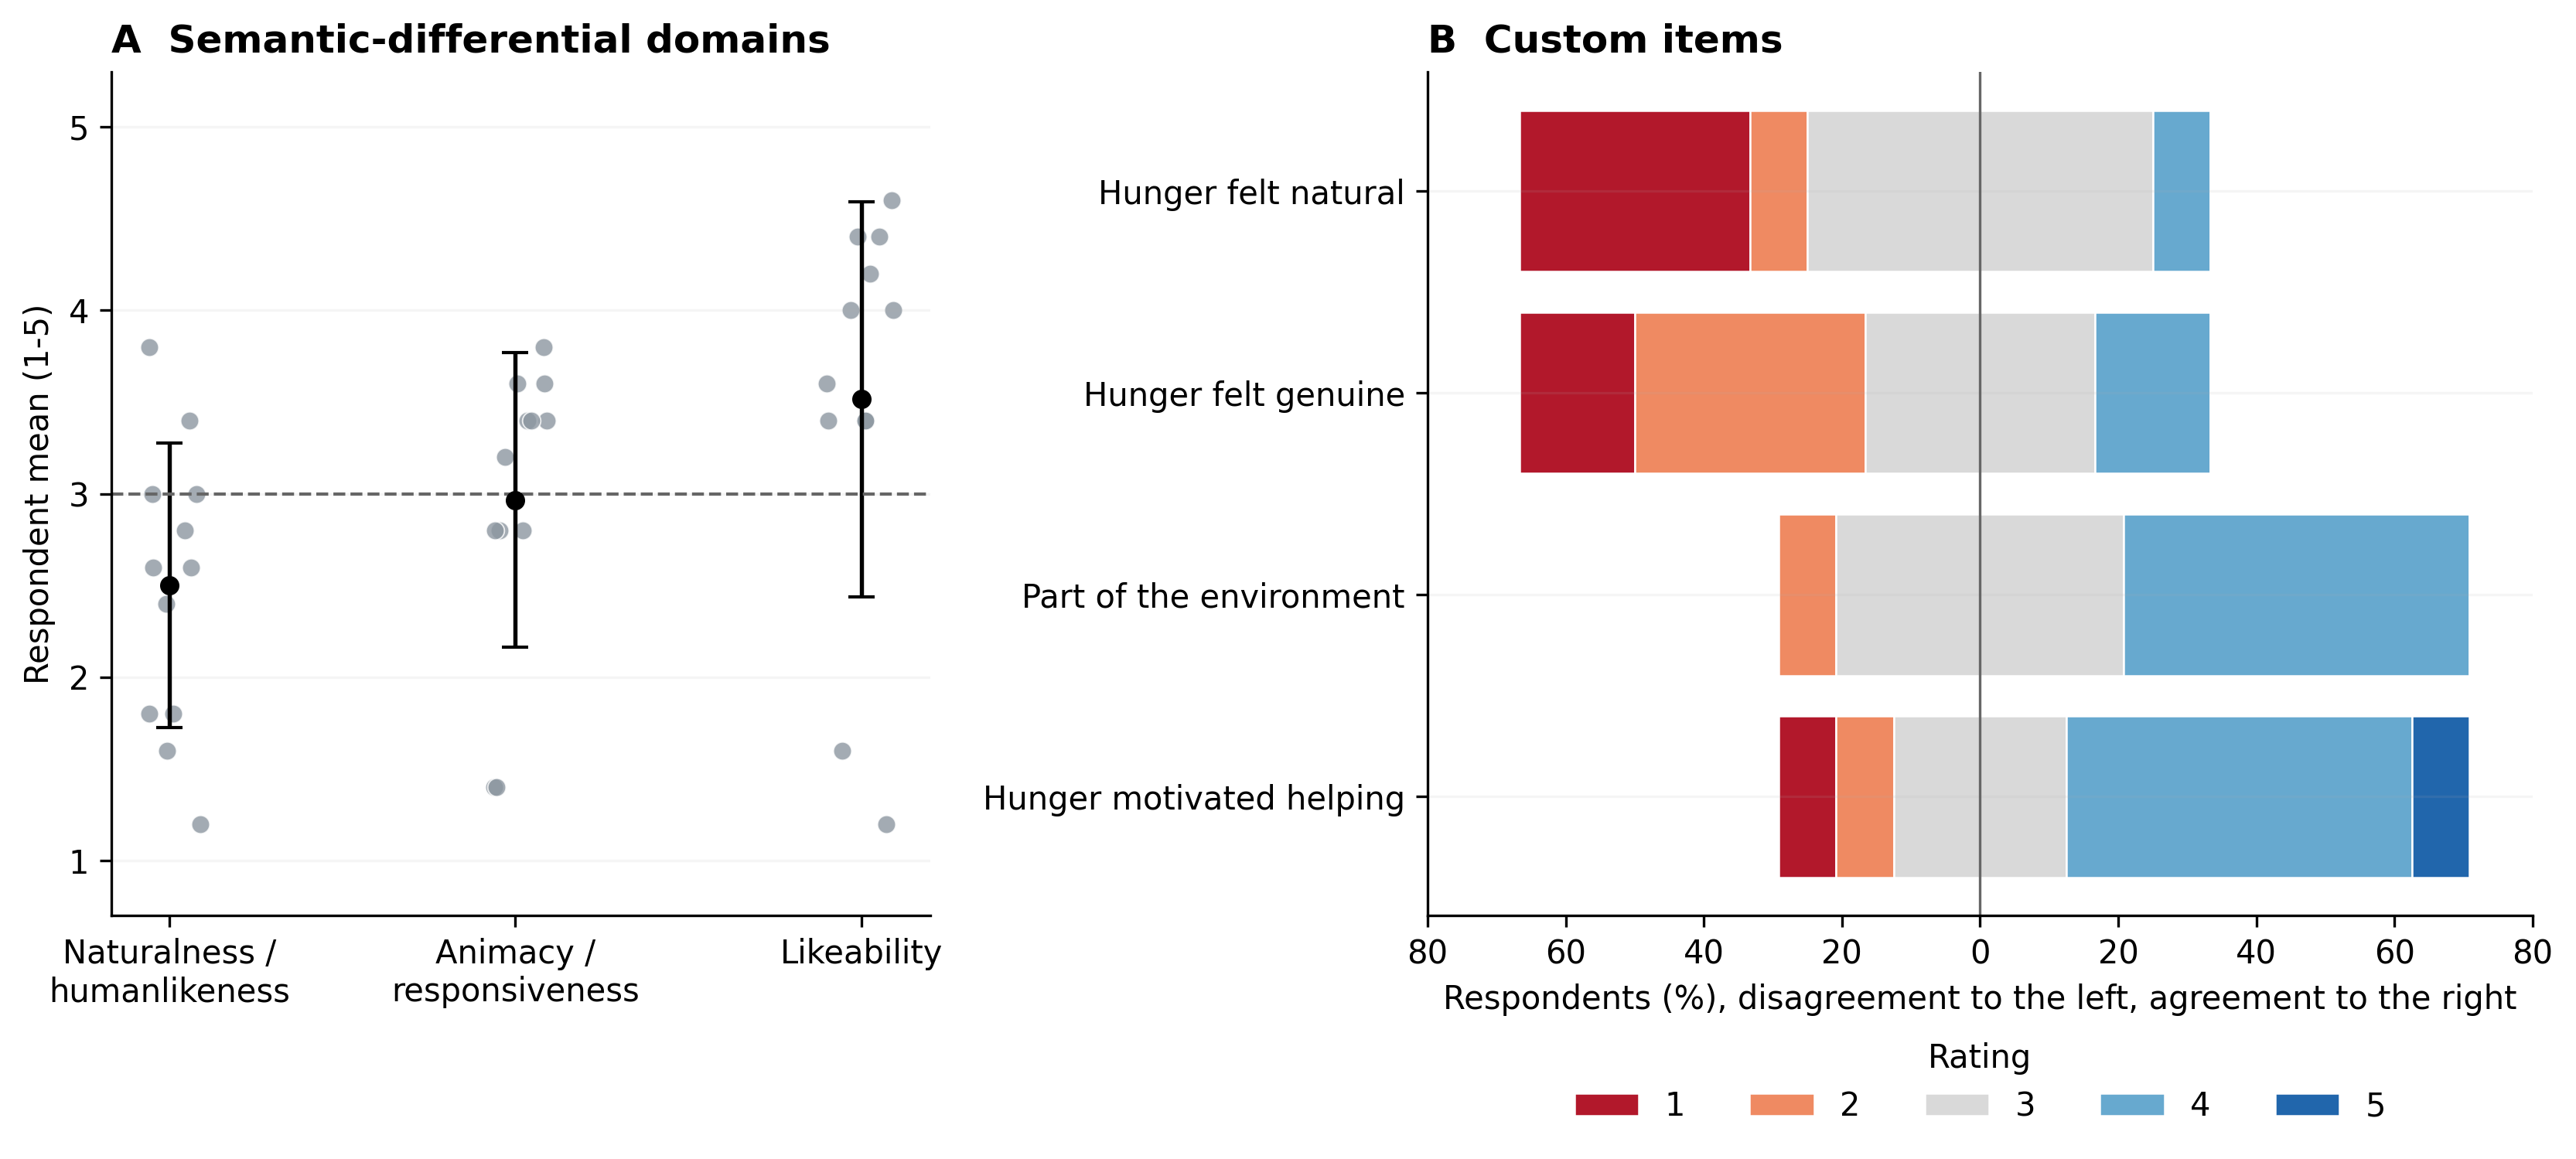
\includegraphics[width=0.94\textwidth,height=0.42\textheight,keepaspectratio]{Results/Figures/rq4-profile.png}
    \caption[Semantic-differential domains and custom items.]{How the \CoreCohortN{} respondents judged the robot and its hunger (RQ4). Panel A shows each respondent's mean on the three semantic-differential domains, with the group mean and standard deviation and a dashed line at the neutral midpoint of 3. Panel B shows every answer to the four custom items, from 1 (dark red, strong disagreement) to 5 (dark blue, strong agreement), with each bar centred on its neutral ratings.}
    \label{fig:results-rq4-profile}
\end{figure}

Figure~\ref{fig:results-rq4-words} shows the twelve nine-point word associations. \emph{Happy} was the only descriptor above the midpoint of 5 ($M=\CoreRosasHappyMean$). The other social and emotional words sat below it: \emph{Social} (\CoreRosasSocialMean), \emph{Feeling} (\CoreRosasFeelingMean), \emph{Emotional} (\CoreRosasEmotionalMean) and \emph{Compassionate} (\CoreRosasCompassionateMean). Threat-related descriptors were near the floor: \emph{Aggressive} ($M=\CoreRosasAggressiveMean$), \emph{Dangerous} (\CoreRosasDangerousMean) and \emph{Scary} (\CoreRosasScaryMean). \emph{Strange} and \emph{Awkward} both averaged \CoreRosasStrangeMean, close to \emph{Social}. Participants saw a happy, harmless robot, but not a strongly social or emotional one, and found it about as strange as it was social.

\begin{figure}[htbp]
    \centering
    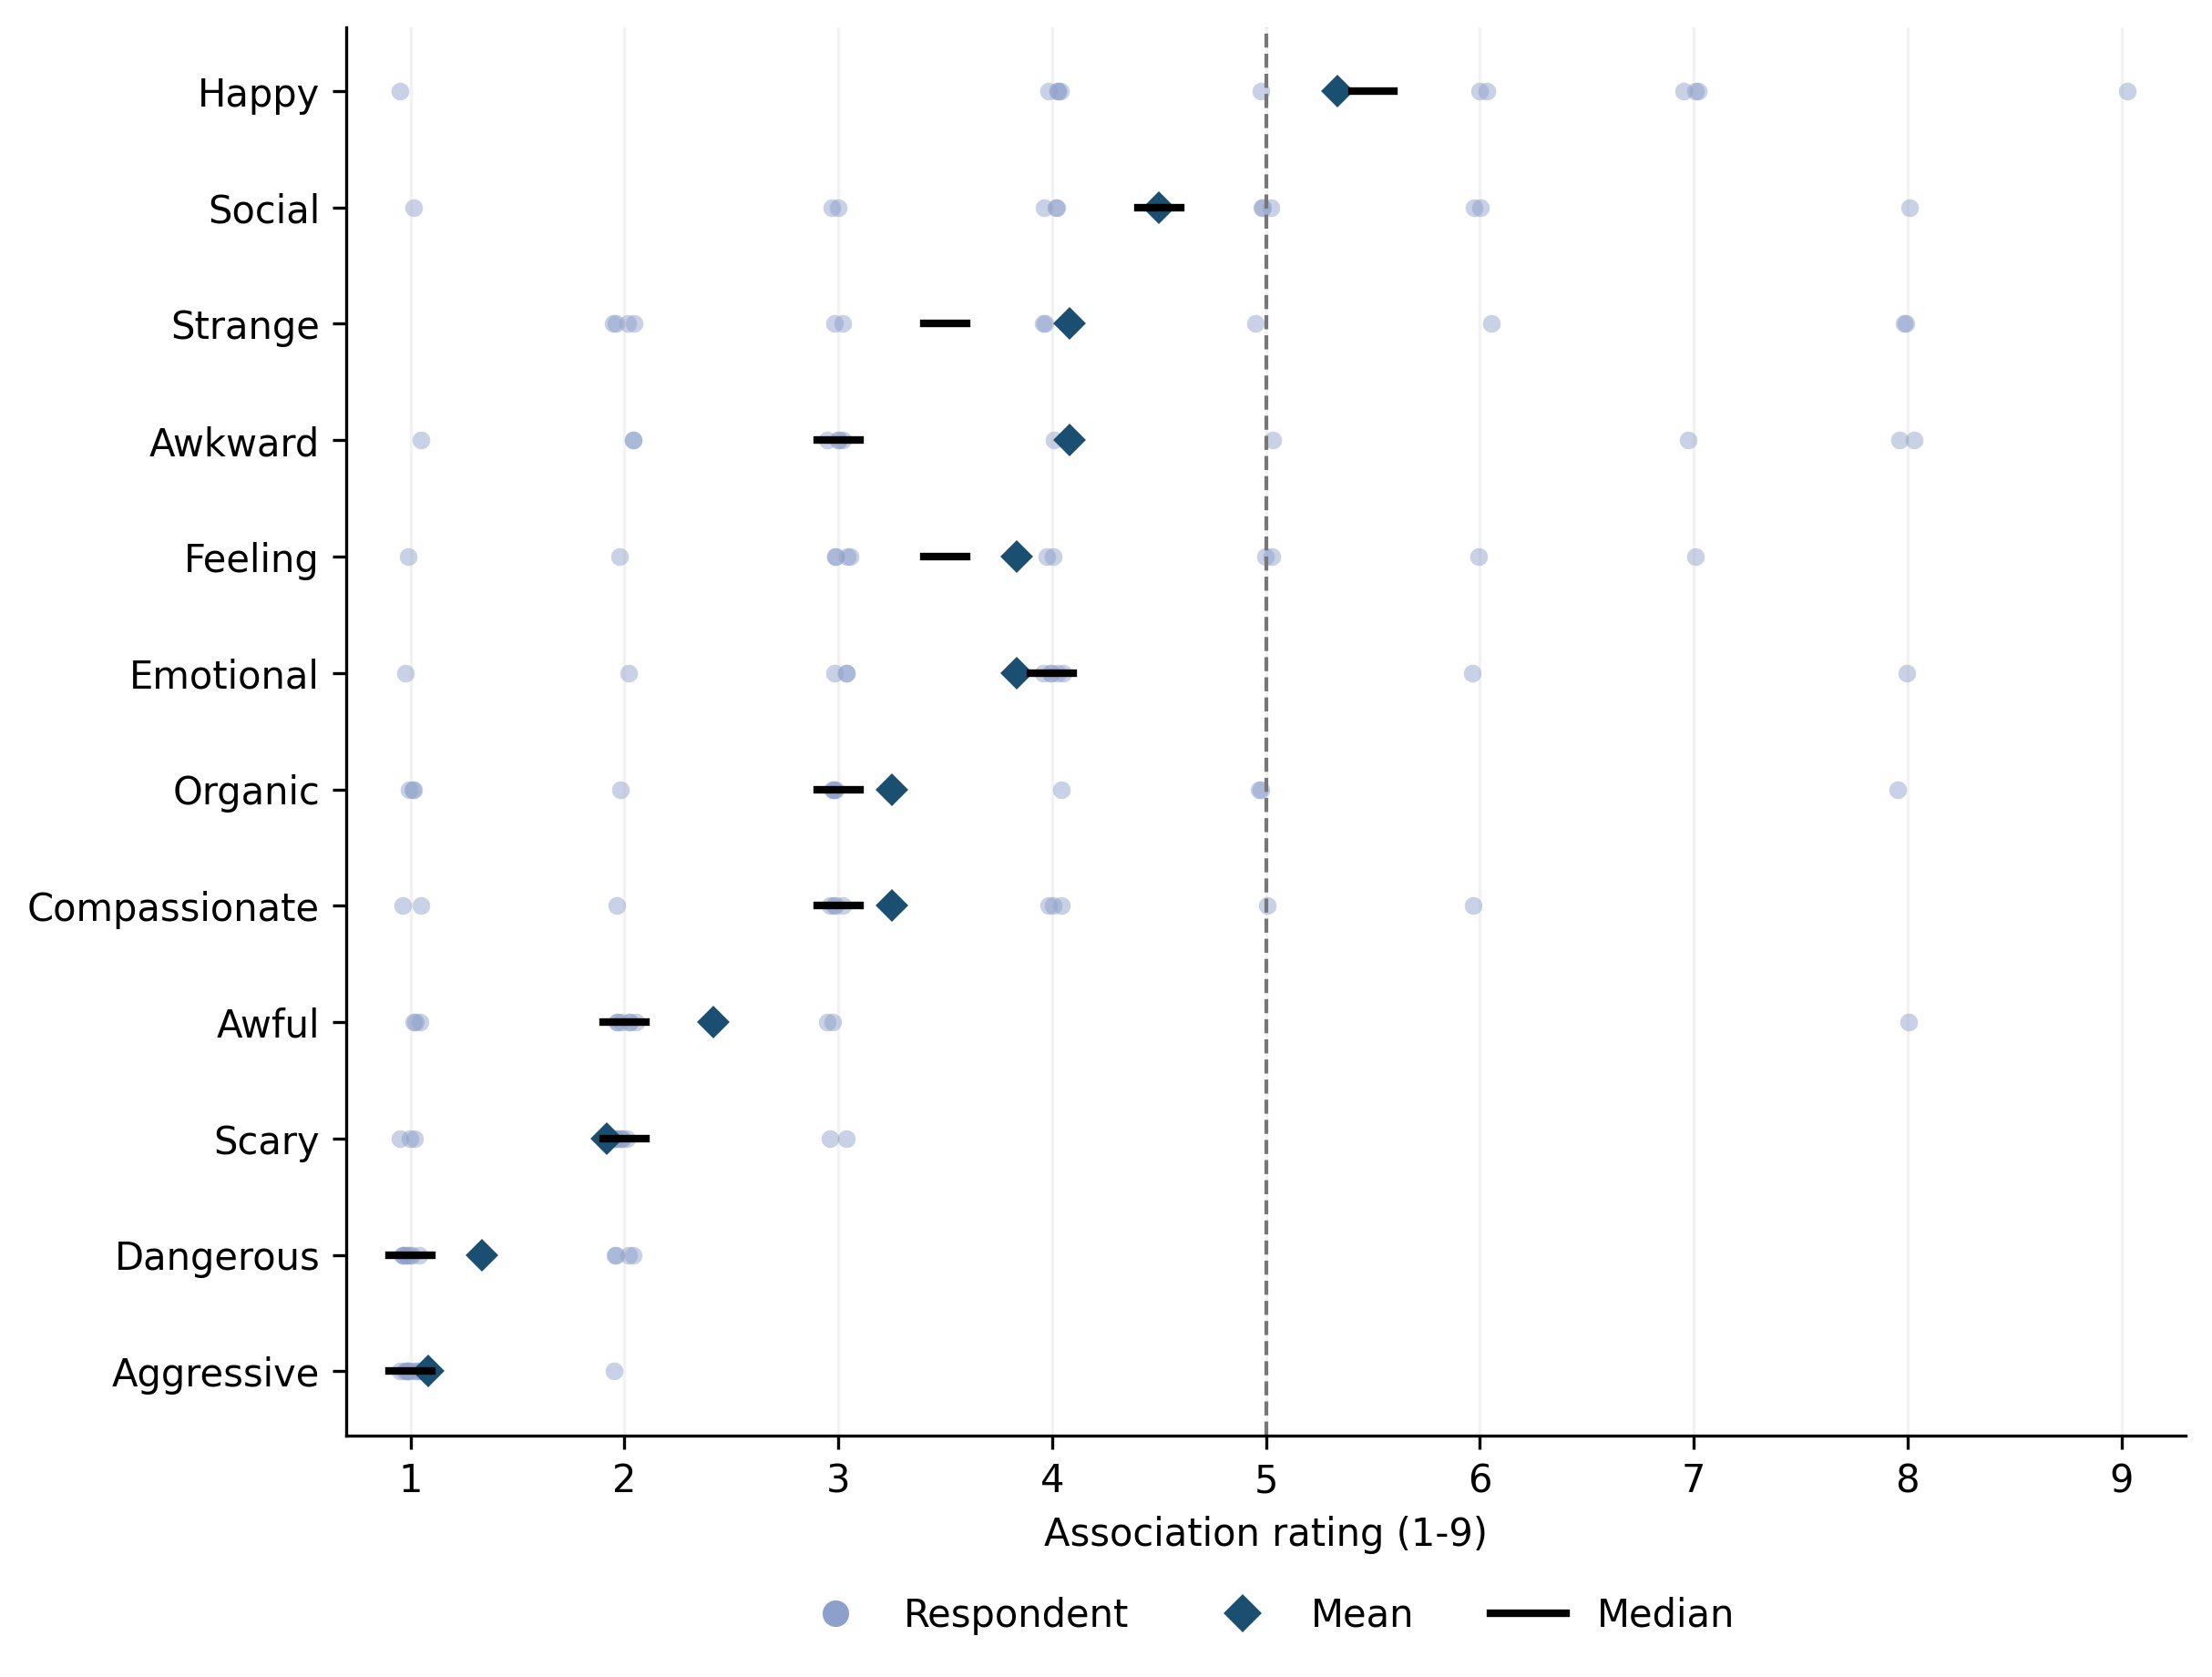
\includegraphics[width=0.78\textwidth,height=0.52\textheight,keepaspectratio]{Results/Figures/rq4-word-associations.png}
    \caption[Word-association ratings by respondent.]{The twelve RoSAS descriptors on their nine-point scale, ordered by mean, with light markers for individual ratings, diamonds for means and bars for medians. The dashed line marks the midpoint of 5. Only \emph{Happy} lies above it, and the threat words sit near the floor.}
    \label{fig:results-rq4-words}
\end{figure}

\subsection{Interpretation of the orexigenic drive}

Only \CoreCustomHungerNaturalAgreement{} of \CoreCohortN{} respondents found the hunger expression natural and \CoreCustomHungerGenuineAgreement{} found it genuine, although \CoreCustomHungerHelpingAgreement{} respondents agreed that it motivated helping and \CoreCustomPartOfEnvironmentAgreement{} felt the robot was part of the environment (Table~\ref{tab:rq4-perception}). For none of the four custom items was the balance between agreement and disagreement significant after Holm correction (all adjusted $p\geq\CoreCustomPartOfEnvironmentPHolm$). One respondent reported being unable to interact with the robot despite completing the ratings. Excluding that record left the descriptive pattern unchanged, and no test became significant (smallest adjusted $p=\CoreSensitivityMinPHolm$).

Within respondents, helping motivation exceeded hunger naturalness by a mean of \CorePairedMeanDifference{} scale points (SD = \CorePairedSDDifference{}; median = \CorePairedMedianDifference). Across the cohort, \CorePairedHigher{} respondents rated helping motivation higher, \CorePairedLower{} rated it lower, and \CorePairedEqual{} gave equal ratings. This paired difference was significant in an exploratory permutation Wilcoxon signed-rank test ($W=\CorePairedW$, $p=\CorePairedP$, rank-biserial $r=\CorePairedRankBiserial$). It also held against perceived genuineness ($p=\CorePairedGenuineP$) and without the respondent who could not interact ($p=\CorePairedSensitivityP$). Participants reported more motivation to help the robot than belief that its hunger was natural.

\begin{table}[htbp]
    \centering
    \small
    \caption[Perceptions of hunger and environmental integration.]{Custom ratings on a five-point scale ($N=\CoreCohortN$). Agreement denotes ratings of 4--5. For the exact sign tests against 3, $B$ counts ratings above 3 and $n_{\mathrm{eff}}$ excludes neutral responses; $p_{\mathrm{Holm}}$ adjusts across the four tests.}
    \label{tab:rq4-perception}
    \begin{tabular}{@{}lrrrr@{}}
        \toprule
        \textbf{Item} & \textbf{M (SD)} & \textbf{Agreement} & $B/n_{\mathrm{eff}}$ & $p_{\mathrm{Holm}}$ \\
        \midrule
        Hunger felt natural & \CoreCustomHungerNaturalMean{} (\CoreCustomHungerNaturalSD{}) & \CoreCustomHungerNaturalAgreement/\CoreCohortN & \CoreCustomHungerNaturalAbove/\CoreCustomHungerNaturalNEff & \CoreCustomHungerNaturalPHolm \\
        Hunger felt genuine & \CoreCustomHungerGenuineMean{} (\CoreCustomHungerGenuineSD{}) & \CoreCustomHungerGenuineAgreement/\CoreCohortN & \CoreCustomHungerGenuineAbove/\CoreCustomHungerGenuineNEff & \CoreCustomHungerGenuinePHolm \\
        Part of the environment & \CoreCustomPartOfEnvironmentMean{} (\CoreCustomPartOfEnvironmentSD{}) & \CoreCustomPartOfEnvironmentAgreement/\CoreCohortN & \CoreCustomPartOfEnvironmentAbove/\CoreCustomPartOfEnvironmentNEff & \CoreCustomPartOfEnvironmentPHolm \\
        Hunger motivated helping & \CoreCustomHungerHelpingMean{} (\CoreCustomHungerHelpingSD{}) & \CoreCustomHungerHelpingAgreement/\CoreCohortN & \CoreCustomHungerHelpingAbove/\CoreCustomHungerHelpingNEff & \CoreCustomHungerHelpingPHolm \\
        \bottomrule
    \end{tabular}
\end{table}

Open responses fell into two groups. Positive accounts centred on personalisation and presence: one participant found face recognition across the room unexpectedly natural, another noted that the robot remembered them across sessions, and two more were caught off guard by a spontaneous joke and by an attentive follow-up question. Negative accounts concentrated on hunger expression, which \CoreHungerCriticisms{} respondents found repetitive, poorly timed or conceptually incoherent. One described a food request that arrived mid-discussion of an ethical dilemma and broke its seriousness. A second reported an urgent Telegram request that turned into reassurance the moment feeding was declined, and objected that the robot's cheerful affect never changed with its hunger state, which left the drive invisible. A third found the requests insistent and saw no reason a robot should be hungry at all, and a fourth judged the hunger state less natural than the rest of the behaviour. Two respondents called the Telegram requests rude, one objecting to their capital letters. These accounts match the measured gap between helping motivation and hunger naturalness.

No association between baseline NARS scores and the post-interaction ratings survived correction. Across the three semantic-differential domains and four custom items, Spearman correlations with overall negative attitudes ranged from $\rho=\CoreNarsRhoMin$ to $\CoreNarsRhoMax$; none survived Holm correction (all $p_{\mathrm{Holm}}\geq\CoreNarsMinPHolm$).

\paragraph{Answer to RQ4.} The orexigenic drive made the robot's need actionable without making it credible. Helping motivation exceeded perceived hunger naturalness, and the written accounts traced the gap to repetitive requests, badly timed interruptions and a cheerful affect that did not change with urgency. Participants nevertheless leaned toward liking the robot and rated it harmless, and \CoreCustomPartOfEnvironmentAgreement{} of \CoreCohortN{} counted it as part of the office.
